\documentclass[twoside]{book}

% Packages required by doxygen
\usepackage{fixltx2e}
\usepackage{calc}
\usepackage{doxygen}
\usepackage[export]{adjustbox} % also loads graphicx
\usepackage{graphicx}
\usepackage[utf8]{inputenc}
\usepackage{makeidx}
\usepackage{multicol}
\usepackage{multirow}
\PassOptionsToPackage{warn}{textcomp}
\usepackage{textcomp}
\usepackage[nointegrals]{wasysym}
\usepackage[table]{xcolor}

% Font selection
\usepackage[T1]{fontenc}
\usepackage[scaled=.90]{helvet}
\usepackage{courier}
\usepackage{amssymb}
\usepackage{sectsty}
\renewcommand{\familydefault}{\sfdefault}
\allsectionsfont{%
  \fontseries{bc}\selectfont%
  \color{darkgray}%
}
\renewcommand{\DoxyLabelFont}{%
  \fontseries{bc}\selectfont%
  \color{darkgray}%
}
\newcommand{\+}{\discretionary{\mbox{\scriptsize$\hookleftarrow$}}{}{}}

% Page & text layout
\usepackage{geometry}
\geometry{%
  a4paper,%
  top=2.5cm,%
  bottom=2.5cm,%
  left=2.5cm,%
  right=2.5cm%
}
\tolerance=750
\hfuzz=15pt
\hbadness=750
\setlength{\emergencystretch}{15pt}
\setlength{\parindent}{0cm}
\setlength{\parskip}{3ex plus 2ex minus 2ex}
\makeatletter
\renewcommand{\paragraph}{%
  \@startsection{paragraph}{4}{0ex}{-1.0ex}{1.0ex}{%
    \normalfont\normalsize\bfseries\SS@parafont%
  }%
}
\renewcommand{\subparagraph}{%
  \@startsection{subparagraph}{5}{0ex}{-1.0ex}{1.0ex}{%
    \normalfont\normalsize\bfseries\SS@subparafont%
  }%
}
\makeatother

% Headers & footers
\usepackage{fancyhdr}
\pagestyle{fancyplain}
\fancyhead[LE]{\fancyplain{}{\bfseries\thepage}}
\fancyhead[CE]{\fancyplain{}{}}
\fancyhead[RE]{\fancyplain{}{\bfseries\leftmark}}
\fancyhead[LO]{\fancyplain{}{\bfseries\rightmark}}
\fancyhead[CO]{\fancyplain{}{}}
\fancyhead[RO]{\fancyplain{}{\bfseries\thepage}}
\fancyfoot[LE]{\fancyplain{}{}}
\fancyfoot[CE]{\fancyplain{}{}}
\fancyfoot[RE]{\fancyplain{}{\bfseries\scriptsize Generated by Doxygen }}
\fancyfoot[LO]{\fancyplain{}{\bfseries\scriptsize Generated by Doxygen }}
\fancyfoot[CO]{\fancyplain{}{}}
\fancyfoot[RO]{\fancyplain{}{}}
\renewcommand{\footrulewidth}{0.4pt}
\renewcommand{\chaptermark}[1]{%
  \markboth{#1}{}%
}
\renewcommand{\sectionmark}[1]{%
  \markright{\thesection\ #1}%
}

% Indices & bibliography
\usepackage{natbib}
\usepackage[titles]{tocloft}
\setcounter{tocdepth}{3}
\setcounter{secnumdepth}{5}
\makeindex

% Hyperlinks (required, but should be loaded last)
\usepackage{ifpdf}
\ifpdf
  \usepackage[pdftex,pagebackref=true]{hyperref}
\else
  \usepackage[ps2pdf,pagebackref=true]{hyperref}
\fi
\hypersetup{%
  colorlinks=true,%
  linkcolor=blue,%
  citecolor=blue,%
  unicode%
}

% Custom commands
\newcommand{\clearemptydoublepage}{%
  \newpage{\pagestyle{empty}\cleardoublepage}%
}

\usepackage{caption}
\captionsetup{labelsep=space,justification=centering,font={bf},singlelinecheck=off,skip=4pt,position=top}

%===== C O N T E N T S =====

\begin{document}

% Titlepage & ToC
\hypersetup{pageanchor=false,
             bookmarksnumbered=true,
             pdfencoding=unicode
            }
\pagenumbering{alph}
\begin{titlepage}
\vspace*{7cm}
\begin{center}%
{\Large Traveller\textquotesingle{}s app }\\
\vspace*{1cm}
{\large Generated by Doxygen 1.8.13}\\
\end{center}
\end{titlepage}
\clearemptydoublepage
\pagenumbering{roman}
\tableofcontents
\clearemptydoublepage
\pagenumbering{arabic}
\hypersetup{pageanchor=true}

%--- Begin generated contents ---
\chapter{About Project}
\label{index}\hypertarget{index}{}\hypertarget{index_First}{}\section{Project\textquotesingle{}s aim}\label{index_First}
The air of this project is to create an application to save information for different trips. In order to use the application every user should create his own profile by registering\mbox{[}saving his personal data(username, password and email) to a database\mbox{]}. After registering a personal database must be created where all trips of the user will be saved. Every trip should have a destination(location), time period, grade(between 1-\/5), comment and photos. Also every user can have friends with whom he can share information. Moreover he can see where his friends have been and what was their impression of the trip(grade and comment).\hypertarget{index_Github}{}\subsection{Github}\label{index_Github}
\href{https://github.com/bdimitrow/TravellersApp}{\tt https\+://github.\+com/bdimitrow/\+Travellers\+App}\hypertarget{index_Second}{}\section{Happy path}\label{index_Second}

\begin{DoxyItemize}
\item The \char`\"{}create a profile\char`\"{} scenario happens just in case the username and the email are not already taken. ~\newline

\item The \char`\"{}logging in\char`\"{} scenario happens only when existing username and matching it password are entered. ~\newline
 
\end{DoxyItemize}\hypertarget{index_running}{}\subsection{Run the program}\label{index_running}
Output\+: Welcome to Traveller\textquotesingle{}s Аpp!
\begin{DoxyEnumerate}
\item Register
\item Login
\item Exit ~\newline
 Choose an action\+: 
\end{DoxyEnumerate}\hypertarget{index_create}{}\subsection{Create a profile}\label{index_create}
Input\+: 1~\newline
 Output\+: Enter a username\+:~\newline
 Input\+: testusername~\newline
 Output\+: Enter a password\+:~\newline
 Input\+: parolae43~\newline
 Output\+: Enter an email\+:~\newline
 Input\+: testde.\+bg~\newline
 Output\+: You have been successfully registered!\hypertarget{index_login}{}\subsection{Logging in}\label{index_login}
Input\+: 2~\newline
 Output\+: Enter a username\+: ~\newline
 Input\+: testusername~\newline
 Output\+: Enter a password\+: ~\newline
 Input\+: parolatae43 ~\newline
 Output\+: Successfully logged in! ~\newline
 ~\newline
 The menu\+Logged is displayed now! ~\newline
 
\chapter{Class Index}
\section{Class List}
Here are the classes, structs, unions and interfaces with brief descriptions\+:\begin{DoxyCompactList}
\item\contentsline{section}{\hyperlink{class_date}{Date} \\*A date class }{\pageref{class_date}}{}
\item\contentsline{section}{\hyperlink{class_destination}{Destination} \\*A destination class }{\pageref{class_destination}}{}
\item\contentsline{section}{\hyperlink{class_user}{User} \\*A user class }{\pageref{class_user}}{}
\end{DoxyCompactList}

\chapter{File Index}
\section{File List}
Here is a list of all files with brief descriptions\+:\begin{DoxyCompactList}
\item\contentsline{section}{\hyperlink{application_8h}{application.\+h} }{\pageref{application_8h}}{}
\item\contentsline{section}{\hyperlink{date_8cpp}{date.\+cpp} }{\pageref{date_8cpp}}{}
\item\contentsline{section}{\hyperlink{date_8h}{date.\+h} }{\pageref{date_8h}}{}
\item\contentsline{section}{\hyperlink{destination_8cpp}{destination.\+cpp} }{\pageref{destination_8cpp}}{}
\item\contentsline{section}{\hyperlink{destination_8h}{destination.\+h} }{\pageref{destination_8h}}{}
\item\contentsline{section}{\hyperlink{main_8cpp}{main.\+cpp} }{\pageref{main_8cpp}}{}
\item\contentsline{section}{\hyperlink{menus_8h}{menus.\+h} }{\pageref{menus_8h}}{}
\item\contentsline{section}{\hyperlink{read_file_8h}{read\+File.\+h} }{\pageref{read_file_8h}}{}
\item\contentsline{section}{\hyperlink{user_8cpp}{user.\+cpp} }{\pageref{user_8cpp}}{}
\item\contentsline{section}{\hyperlink{user_8h}{user.\+h} }{\pageref{user_8h}}{}
\end{DoxyCompactList}

\chapter{Class Documentation}
\hypertarget{class_date}{}\section{Date Class Reference}
\label{class_date}\index{Date@{Date}}


A date class.  




{\ttfamily \#include $<$date.\+h$>$}



Collaboration diagram for Date\+:\nopagebreak
\begin{figure}[H]
\begin{center}
\leavevmode
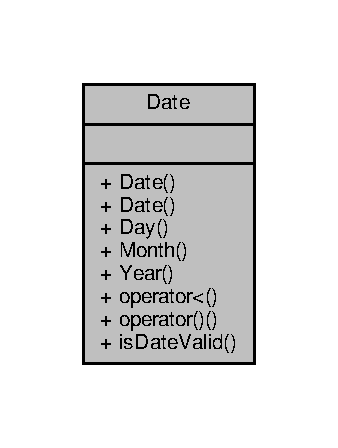
\includegraphics[width=162pt]{class_date__coll__graph}
\end{center}
\end{figure}
\subsection*{Public Member Functions}
\begin{DoxyCompactItemize}
\item 
\hyperlink{class_date_a4e59ed4ba66eec61c27460c5d09fa1bd}{Date} ()
\item 
\hyperlink{class_date_af80a5016fde0d599f0a15900193fc663}{Date} (int, int, int)
\item 
int \hyperlink{class_date_ad7f2e4e42aadc85322503dbef8484ad5}{Day} () const
\item 
int \hyperlink{class_date_a1c1871e2d6adcb08fd30ffae440b3803}{Month} () const
\item 
int \hyperlink{class_date_a284f8985596b83ad9388b464eb6b54bd}{Year} () const
\item 
bool \hyperlink{class_date_a08c0538091d061550b90787d9313ca61}{operator$<$} (const \hyperlink{class_date}{Date} \&) const
\item 
\hyperlink{class_date}{Date} \hyperlink{class_date_a425bd02efac05e6b65a8b7456317822f}{operator()} (int y, int m, int d)
\item 
bool \hyperlink{class_date_a2d9a87adab3ae18acdb13e027ad1d0aa}{is\+Date\+Valid} (const \hyperlink{class_date}{Date} \&)
\end{DoxyCompactItemize}
\subsection*{Private Attributes}
\begin{DoxyCompactItemize}
\item 
int \hyperlink{class_date_a5b192adcabf2b2871e3f0b76c1ec1601}{day}
\item 
int \hyperlink{class_date_a533843e07c6ac8d19fee9b16f5336ba2}{month}
\item 
int \hyperlink{class_date_a3eeced2ed56bc95d56782b9e738db8ea}{year}
\end{DoxyCompactItemize}
\subsection*{Friends}
\begin{DoxyCompactItemize}
\item 
ostream \& \hyperlink{class_date_affced1a8a8f9f0e9dd009af0a22dfe33}{operator$<$$<$} (ostream \&fout, const \hyperlink{class_date}{Date} \&dt)
\end{DoxyCompactItemize}


\subsection{Detailed Description}
A date class. 


\begin{DoxyParams}{Parameters}
{\em day} & is an integer \\
\hline
{\em month} & is an integer \\
\hline
{\em year} & is an integer\\
\hline
\end{DoxyParams}
This class is used to initialize dates. They are required to describe the duration of a trip. We initialize a period with two dates\+: starting date and ending date. 

\subsection{Constructor \& Destructor Documentation}
\mbox{\Hypertarget{class_date_a4e59ed4ba66eec61c27460c5d09fa1bd}\label{class_date_a4e59ed4ba66eec61c27460c5d09fa1bd}} 
\index{Date@{Date}!Date@{Date}}
\index{Date@{Date}!Date@{Date}}
\subsubsection{\texorpdfstring{Date()}{Date()}\hspace{0.1cm}{\footnotesize\ttfamily [1/2]}}
{\footnotesize\ttfamily Date\+::\+Date (\begin{DoxyParamCaption}{ }\end{DoxyParamCaption})\hspace{0.3cm}{\ttfamily [inline]}}

A default constructor. Here is the call graph for this function\+:\nopagebreak
\begin{figure}[H]
\begin{center}
\leavevmode
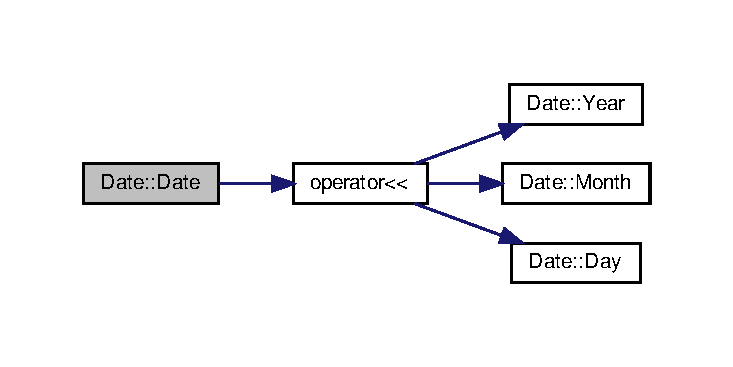
\includegraphics[width=350pt]{class_date_a4e59ed4ba66eec61c27460c5d09fa1bd_cgraph}
\end{center}
\end{figure}
\mbox{\Hypertarget{class_date_af80a5016fde0d599f0a15900193fc663}\label{class_date_af80a5016fde0d599f0a15900193fc663}} 
\index{Date@{Date}!Date@{Date}}
\index{Date@{Date}!Date@{Date}}
\subsubsection{\texorpdfstring{Date()}{Date()}\hspace{0.1cm}{\footnotesize\ttfamily [2/2]}}
{\footnotesize\ttfamily Date\+::\+Date (\begin{DoxyParamCaption}\item[{int}]{y,  }\item[{int}]{m,  }\item[{int}]{d }\end{DoxyParamCaption})}

A parametrized constructor. 

\subsection{Member Function Documentation}
\mbox{\Hypertarget{class_date_ad7f2e4e42aadc85322503dbef8484ad5}\label{class_date_ad7f2e4e42aadc85322503dbef8484ad5}} 
\index{Date@{Date}!Day@{Day}}
\index{Day@{Day}!Date@{Date}}
\subsubsection{\texorpdfstring{Day()}{Day()}}
{\footnotesize\ttfamily int Date\+::\+Day (\begin{DoxyParamCaption}{ }\end{DoxyParamCaption}) const}

Method setting the day. Here is the caller graph for this function\+:\nopagebreak
\begin{figure}[H]
\begin{center}
\leavevmode
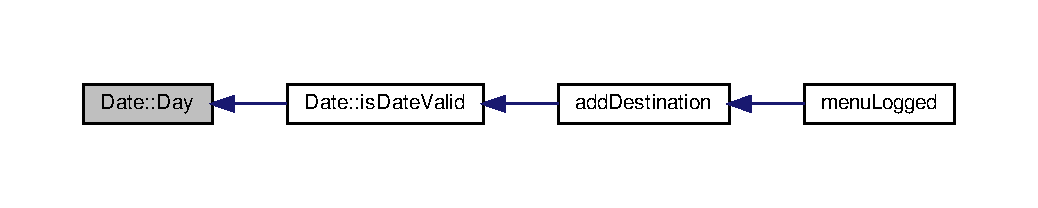
\includegraphics[width=350pt]{class_date_ad7f2e4e42aadc85322503dbef8484ad5_icgraph}
\end{center}
\end{figure}
\mbox{\Hypertarget{class_date_a2d9a87adab3ae18acdb13e027ad1d0aa}\label{class_date_a2d9a87adab3ae18acdb13e027ad1d0aa}} 
\index{Date@{Date}!is\+Date\+Valid@{is\+Date\+Valid}}
\index{is\+Date\+Valid@{is\+Date\+Valid}!Date@{Date}}
\subsubsection{\texorpdfstring{is\+Date\+Valid()}{isDateValid()}}
{\footnotesize\ttfamily bool Date\+::is\+Date\+Valid (\begin{DoxyParamCaption}\item[{const \hyperlink{class_date}{Date} \&}]{date }\end{DoxyParamCaption})}

This function accepts an object ot type \hyperlink{class_date}{Date} and determines whether the date is valid(2020.\+13.\+14 is an invalid date). 
\begin{DoxyParams}{Parameters}
{\em \hyperlink{class_date}{Date}} & date\+To\+Be\+Checked \\
\hline
\end{DoxyParams}
\begin{DoxyReturn}{Returns}
true or false. 
\end{DoxyReturn}
Here is the call graph for this function\+:\nopagebreak
\begin{figure}[H]
\begin{center}
\leavevmode
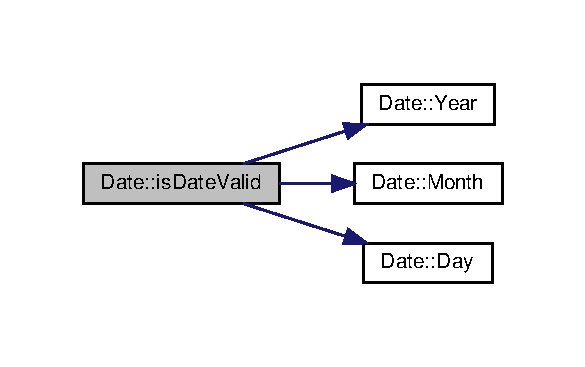
\includegraphics[width=281pt]{class_date_a2d9a87adab3ae18acdb13e027ad1d0aa_cgraph}
\end{center}
\end{figure}
Here is the caller graph for this function\+:\nopagebreak
\begin{figure}[H]
\begin{center}
\leavevmode
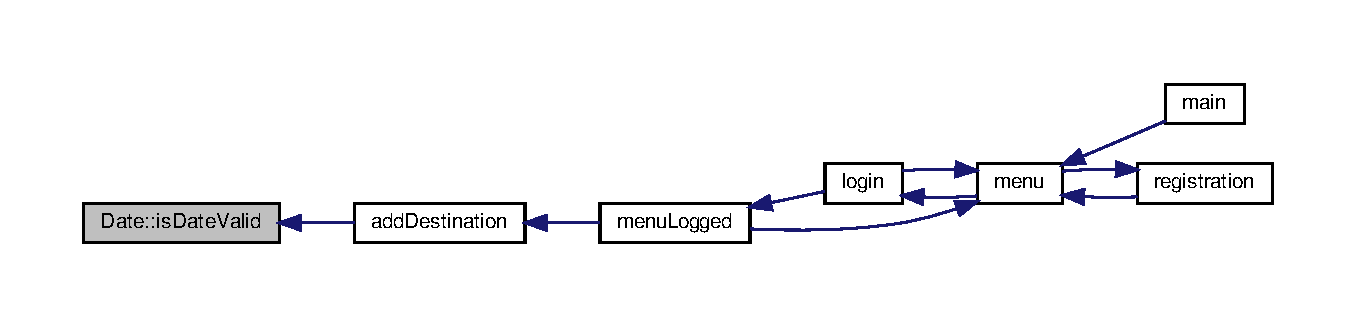
\includegraphics[width=350pt]{class_date_a2d9a87adab3ae18acdb13e027ad1d0aa_icgraph}
\end{center}
\end{figure}
\mbox{\Hypertarget{class_date_a1c1871e2d6adcb08fd30ffae440b3803}\label{class_date_a1c1871e2d6adcb08fd30ffae440b3803}} 
\index{Date@{Date}!Month@{Month}}
\index{Month@{Month}!Date@{Date}}
\subsubsection{\texorpdfstring{Month()}{Month()}}
{\footnotesize\ttfamily int Date\+::\+Month (\begin{DoxyParamCaption}{ }\end{DoxyParamCaption}) const}

Method setting the month. Here is the caller graph for this function\+:\nopagebreak
\begin{figure}[H]
\begin{center}
\leavevmode
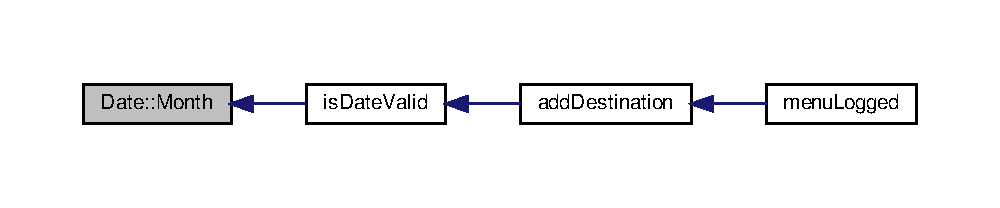
\includegraphics[width=350pt]{class_date_a1c1871e2d6adcb08fd30ffae440b3803_icgraph}
\end{center}
\end{figure}
\mbox{\Hypertarget{class_date_a425bd02efac05e6b65a8b7456317822f}\label{class_date_a425bd02efac05e6b65a8b7456317822f}} 
\index{Date@{Date}!operator()@{operator()}}
\index{operator()@{operator()}!Date@{Date}}
\subsubsection{\texorpdfstring{operator()()}{operator()()}}
{\footnotesize\ttfamily \hyperlink{class_date}{Date} Date\+::operator() (\begin{DoxyParamCaption}\item[{int}]{y,  }\item[{int}]{m,  }\item[{int}]{d }\end{DoxyParamCaption})}

Overloaded operator(). It is setting new date(used in date validation). \mbox{\Hypertarget{class_date_a08c0538091d061550b90787d9313ca61}\label{class_date_a08c0538091d061550b90787d9313ca61}} 
\index{Date@{Date}!operator$<$@{operator$<$}}
\index{operator$<$@{operator$<$}!Date@{Date}}
\subsubsection{\texorpdfstring{operator$<$()}{operator<()}}
{\footnotesize\ttfamily bool Date\+::operator$<$ (\begin{DoxyParamCaption}\item[{const \hyperlink{class_date}{Date} \&}]{other }\end{DoxyParamCaption}) const}

A bool method comparing two dates. \mbox{\Hypertarget{class_date_a284f8985596b83ad9388b464eb6b54bd}\label{class_date_a284f8985596b83ad9388b464eb6b54bd}} 
\index{Date@{Date}!Year@{Year}}
\index{Year@{Year}!Date@{Date}}
\subsubsection{\texorpdfstring{Year()}{Year()}}
{\footnotesize\ttfamily int Date\+::\+Year (\begin{DoxyParamCaption}{ }\end{DoxyParamCaption}) const}

Method setting the year. Here is the caller graph for this function\+:\nopagebreak
\begin{figure}[H]
\begin{center}
\leavevmode
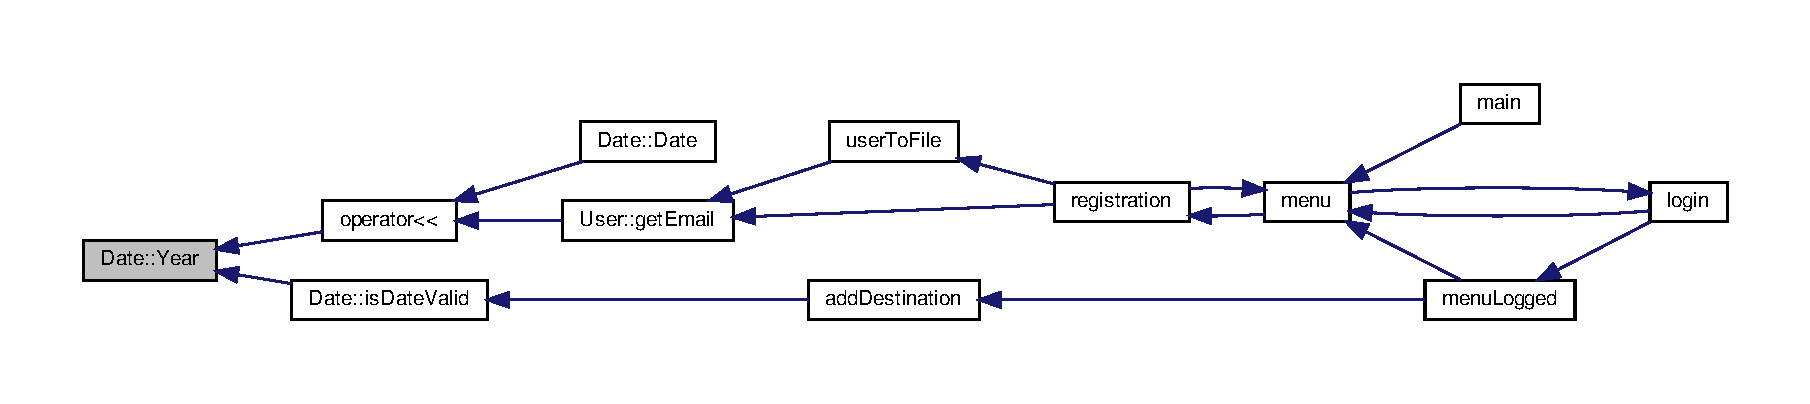
\includegraphics[width=350pt]{class_date_a284f8985596b83ad9388b464eb6b54bd_icgraph}
\end{center}
\end{figure}


\subsection{Friends And Related Function Documentation}
\mbox{\Hypertarget{class_date_affced1a8a8f9f0e9dd009af0a22dfe33}\label{class_date_affced1a8a8f9f0e9dd009af0a22dfe33}} 
\index{Date@{Date}!operator$<$$<$@{operator$<$$<$}}
\index{operator$<$$<$@{operator$<$$<$}!Date@{Date}}
\subsubsection{\texorpdfstring{operator$<$$<$}{operator<<}}
{\footnotesize\ttfamily ostream\& operator$<$$<$ (\begin{DoxyParamCaption}\item[{ostream \&}]{fout,  }\item[{const \hyperlink{class_date}{Date} \&}]{dt }\end{DoxyParamCaption})\hspace{0.3cm}{\ttfamily [friend]}}

Overloaded operator$<$$<$. 

\subsection{Member Data Documentation}
\mbox{\Hypertarget{class_date_a5b192adcabf2b2871e3f0b76c1ec1601}\label{class_date_a5b192adcabf2b2871e3f0b76c1ec1601}} 
\index{Date@{Date}!day@{day}}
\index{day@{day}!Date@{Date}}
\subsubsection{\texorpdfstring{day}{day}}
{\footnotesize\ttfamily int Date\+::day\hspace{0.3cm}{\ttfamily [private]}}

Variable for day. \mbox{\Hypertarget{class_date_a533843e07c6ac8d19fee9b16f5336ba2}\label{class_date_a533843e07c6ac8d19fee9b16f5336ba2}} 
\index{Date@{Date}!month@{month}}
\index{month@{month}!Date@{Date}}
\subsubsection{\texorpdfstring{month}{month}}
{\footnotesize\ttfamily int Date\+::month\hspace{0.3cm}{\ttfamily [private]}}

Variable for month \mbox{\Hypertarget{class_date_a3eeced2ed56bc95d56782b9e738db8ea}\label{class_date_a3eeced2ed56bc95d56782b9e738db8ea}} 
\index{Date@{Date}!year@{year}}
\index{year@{year}!Date@{Date}}
\subsubsection{\texorpdfstring{year}{year}}
{\footnotesize\ttfamily int Date\+::year\hspace{0.3cm}{\ttfamily [private]}}

Variable for year 

The documentation for this class was generated from the following files\+:\begin{DoxyCompactItemize}
\item 
\hyperlink{date_8h}{date.\+h}\item 
\hyperlink{date_8cpp}{date.\+cpp}\end{DoxyCompactItemize}

\hypertarget{class_destination}{}\section{Destination Class Reference}
\label{class_destination}\index{Destination@{Destination}}


A destination class.  




{\ttfamily \#include $<$destination.\+h$>$}



Collaboration diagram for Destination\+:\nopagebreak
\begin{figure}[H]
\begin{center}
\leavevmode
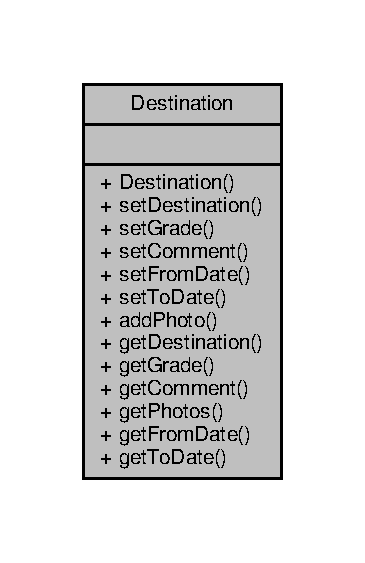
\includegraphics[width=175pt]{class_destination__coll__graph}
\end{center}
\end{figure}
\subsection*{Public Member Functions}
\begin{DoxyCompactItemize}
\item 
\hyperlink{class_destination_ac23f3307b89ac7a8fa8aa8d4ff3e22a6}{Destination} ()
\item 
void \hyperlink{class_destination_a9cafaaf83be9ea548401caf2a2c4d839}{set\+Destination} (string)
\item 
void \hyperlink{class_destination_ac7f1c3be54b5223aa1e9ad4523ef6976}{set\+Grade} (unsigned)
\item 
void \hyperlink{class_destination_a08199ade6e0bf7488d796d85dec8cfd9}{set\+Comment} (string)
\item 
void \hyperlink{class_destination_a6fc539f51a5fd6844fef290facc4e887}{set\+From\+Date} (\hyperlink{class_date}{Date} fr)
\item 
void \hyperlink{class_destination_afec038764d48882a9005cea50e418219}{set\+To\+Date} (\hyperlink{class_date}{Date} t)
\item 
void \hyperlink{class_destination_a6494a9eae34083fd09861ba8f6923e92}{add\+Photo} (const string \&)
\item 
string \hyperlink{class_destination_a6544fb0fa820f5a6b914a38cdcc949f9}{get\+Destination} () const
\item 
unsigned \hyperlink{class_destination_a34dd7a2072743078d5067d336dc3c25d}{get\+Grade} () const
\item 
string \hyperlink{class_destination_a4d20ef4e561fa10dd81561b9cd61c55c}{get\+Comment} () const
\item 
vector$<$ string $>$ \hyperlink{class_destination_ade746815624a6fd5add31a3475e04b45}{get\+Photos} () const
\item 
\hyperlink{class_date}{Date} \hyperlink{class_destination_ac6265579620a20899f5e4cf817d037c8}{get\+From\+Date} () const
\item 
\hyperlink{class_date}{Date} \hyperlink{class_destination_a6a98c7e1c0ffa4b821d3f7dd85cad3dd}{get\+To\+Date} () const
\end{DoxyCompactItemize}
\subsection*{Private Attributes}
\begin{DoxyCompactItemize}
\item 
string \hyperlink{class_destination_ad5bc042020c7faf68d8940061142a0ea}{destination}
\item 
\hyperlink{class_date}{Date} \hyperlink{class_destination_a0dea129cf2457e922c57b7fb5996509a}{from}
\item 
\hyperlink{class_date}{Date} \hyperlink{class_destination_ad556f5592b3bcb4ab407064bc1f0763c}{to}
\item 
unsigned \hyperlink{class_destination_afbab7d354ba8c639501755e48261012e}{grade}
\item 
string \hyperlink{class_destination_a4788b97b93c5336a8717540e0daa841a}{comment}
\item 
vector$<$ string $>$ \hyperlink{class_destination_a17cb8de845ce9d65eb7082c79c617444}{photos}
\end{DoxyCompactItemize}


\subsection{Detailed Description}
A destination class. 


\begin{DoxyParams}{Parameters}
{\em destination} & is type string keeping the location. \\
\hline
{\em from} & is type \hyperlink{class_date}{Date} keeping the start date. \\
\hline
{\em to} & is type \hyperlink{class_date}{Date} keeping the end date. \\
\hline
{\em grade} & is type unsigned. \\
\hline
{\em comment} & is type string. \\
\hline
{\em photos} & is a vector of strings.\\
\hline
\end{DoxyParams}
This class is used to initialize trips. They are part of every user\textquotesingle{}s database. Every trip consists of location, start date, end date, user\textquotesingle{}s grade, user\textquotesingle{}s comment and photos. Class date is used to maintain the dates in class \hyperlink{class_destination}{Destination}. 

\subsection{Constructor \& Destructor Documentation}
\mbox{\Hypertarget{class_destination_ac23f3307b89ac7a8fa8aa8d4ff3e22a6}\label{class_destination_ac23f3307b89ac7a8fa8aa8d4ff3e22a6}} 
\index{Destination@{Destination}!Destination@{Destination}}
\index{Destination@{Destination}!Destination@{Destination}}
\subsubsection{\texorpdfstring{Destination()}{Destination()}}
{\footnotesize\ttfamily Destination\+::\+Destination (\begin{DoxyParamCaption}{ }\end{DoxyParamCaption})\hspace{0.3cm}{\ttfamily [inline]}}

A default constructor. 

\subsection{Member Function Documentation}
\mbox{\Hypertarget{class_destination_a6494a9eae34083fd09861ba8f6923e92}\label{class_destination_a6494a9eae34083fd09861ba8f6923e92}} 
\index{Destination@{Destination}!add\+Photo@{add\+Photo}}
\index{add\+Photo@{add\+Photo}!Destination@{Destination}}
\subsubsection{\texorpdfstring{add\+Photo()}{addPhoto()}}
{\footnotesize\ttfamily void Destination\+::add\+Photo (\begin{DoxyParamCaption}\item[{const string \&}]{new\+Photos }\end{DoxyParamCaption})}

Method adding a phone. Here is the caller graph for this function\+:\nopagebreak
\begin{figure}[H]
\begin{center}
\leavevmode
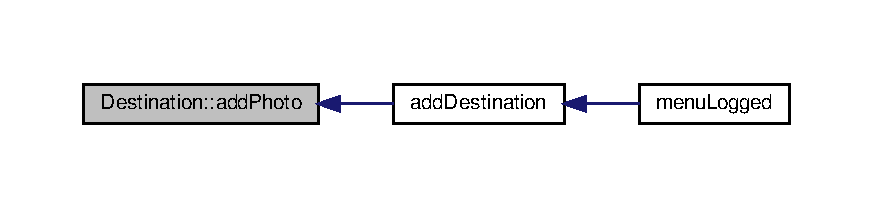
\includegraphics[width=350pt]{class_destination_a6494a9eae34083fd09861ba8f6923e92_icgraph}
\end{center}
\end{figure}
\mbox{\Hypertarget{class_destination_a4d20ef4e561fa10dd81561b9cd61c55c}\label{class_destination_a4d20ef4e561fa10dd81561b9cd61c55c}} 
\index{Destination@{Destination}!get\+Comment@{get\+Comment}}
\index{get\+Comment@{get\+Comment}!Destination@{Destination}}
\subsubsection{\texorpdfstring{get\+Comment()}{getComment()}}
{\footnotesize\ttfamily string Destination\+::get\+Comment (\begin{DoxyParamCaption}{ }\end{DoxyParamCaption}) const\hspace{0.3cm}{\ttfamily [inline]}}

Getter for comment. \begin{DoxyReturn}{Returns}
string comment 
\end{DoxyReturn}
Here is the caller graph for this function\+:\nopagebreak
\begin{figure}[H]
\begin{center}
\leavevmode
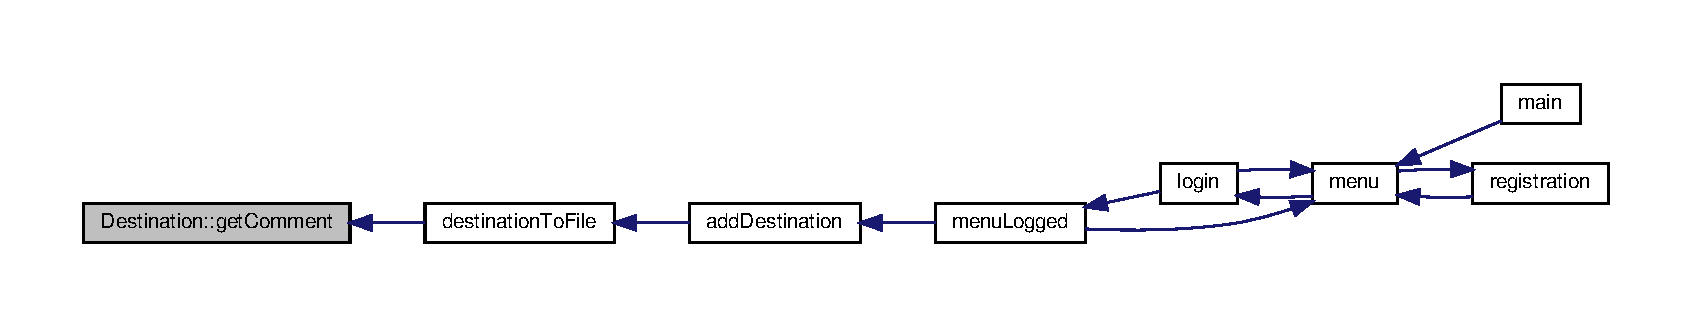
\includegraphics[width=350pt]{class_destination_a4d20ef4e561fa10dd81561b9cd61c55c_icgraph}
\end{center}
\end{figure}
\mbox{\Hypertarget{class_destination_a6544fb0fa820f5a6b914a38cdcc949f9}\label{class_destination_a6544fb0fa820f5a6b914a38cdcc949f9}} 
\index{Destination@{Destination}!get\+Destination@{get\+Destination}}
\index{get\+Destination@{get\+Destination}!Destination@{Destination}}
\subsubsection{\texorpdfstring{get\+Destination()}{getDestination()}}
{\footnotesize\ttfamily string Destination\+::get\+Destination (\begin{DoxyParamCaption}{ }\end{DoxyParamCaption}) const\hspace{0.3cm}{\ttfamily [inline]}}

Getter for destination. \begin{DoxyReturn}{Returns}
string destination 
\end{DoxyReturn}
Here is the caller graph for this function\+:\nopagebreak
\begin{figure}[H]
\begin{center}
\leavevmode
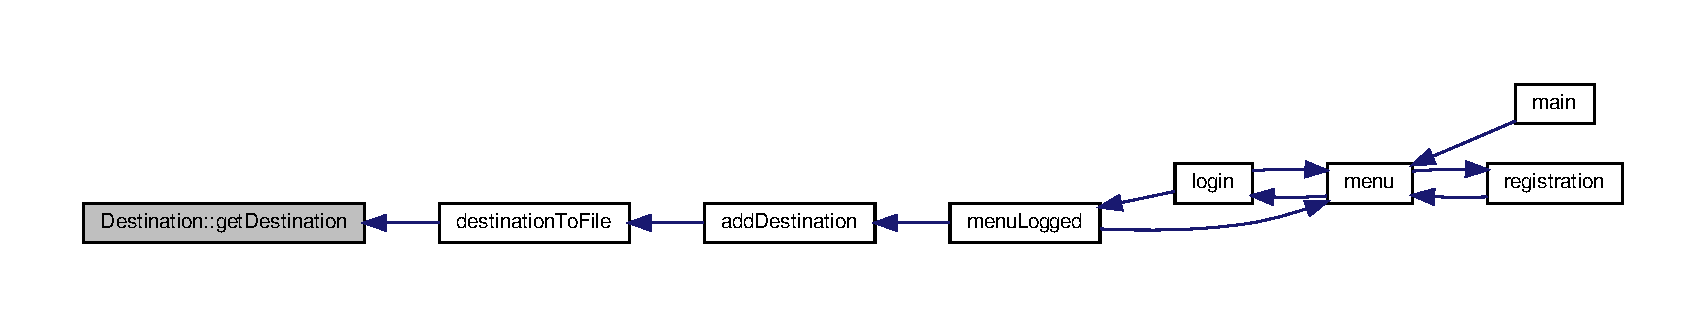
\includegraphics[width=350pt]{class_destination_a6544fb0fa820f5a6b914a38cdcc949f9_icgraph}
\end{center}
\end{figure}
\mbox{\Hypertarget{class_destination_ac6265579620a20899f5e4cf817d037c8}\label{class_destination_ac6265579620a20899f5e4cf817d037c8}} 
\index{Destination@{Destination}!get\+From\+Date@{get\+From\+Date}}
\index{get\+From\+Date@{get\+From\+Date}!Destination@{Destination}}
\subsubsection{\texorpdfstring{get\+From\+Date()}{getFromDate()}}
{\footnotesize\ttfamily \hyperlink{class_date}{Date} Destination\+::get\+From\+Date (\begin{DoxyParamCaption}{ }\end{DoxyParamCaption}) const\hspace{0.3cm}{\ttfamily [inline]}}

Getter for start date. \begin{DoxyReturn}{Returns}
\hyperlink{class_date}{Date} from 
\end{DoxyReturn}
Here is the caller graph for this function\+:\nopagebreak
\begin{figure}[H]
\begin{center}
\leavevmode
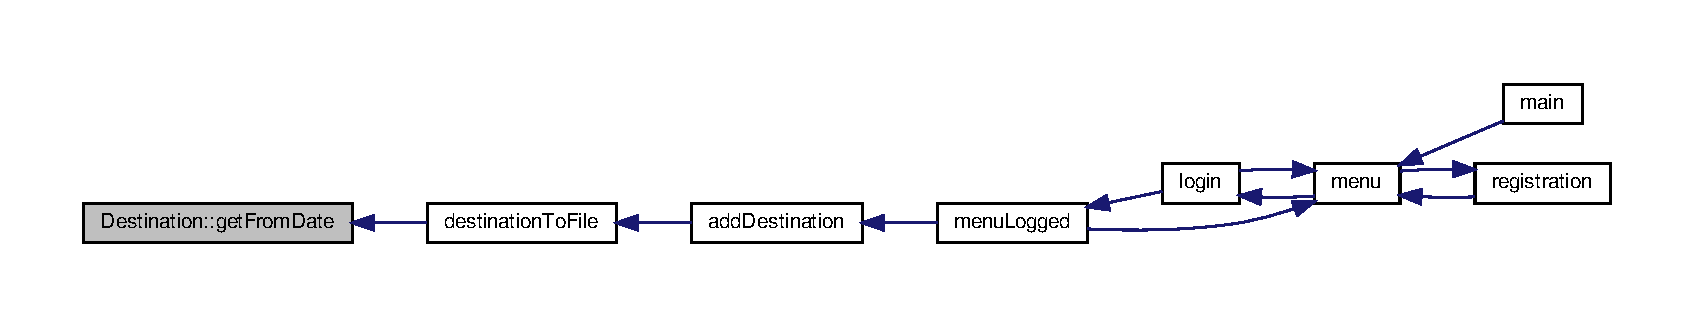
\includegraphics[width=350pt]{class_destination_ac6265579620a20899f5e4cf817d037c8_icgraph}
\end{center}
\end{figure}
\mbox{\Hypertarget{class_destination_a34dd7a2072743078d5067d336dc3c25d}\label{class_destination_a34dd7a2072743078d5067d336dc3c25d}} 
\index{Destination@{Destination}!get\+Grade@{get\+Grade}}
\index{get\+Grade@{get\+Grade}!Destination@{Destination}}
\subsubsection{\texorpdfstring{get\+Grade()}{getGrade()}}
{\footnotesize\ttfamily unsigned Destination\+::get\+Grade (\begin{DoxyParamCaption}{ }\end{DoxyParamCaption}) const\hspace{0.3cm}{\ttfamily [inline]}}

Getter for grade. \begin{DoxyReturn}{Returns}
unsigned grade 
\end{DoxyReturn}
Here is the caller graph for this function\+:\nopagebreak
\begin{figure}[H]
\begin{center}
\leavevmode
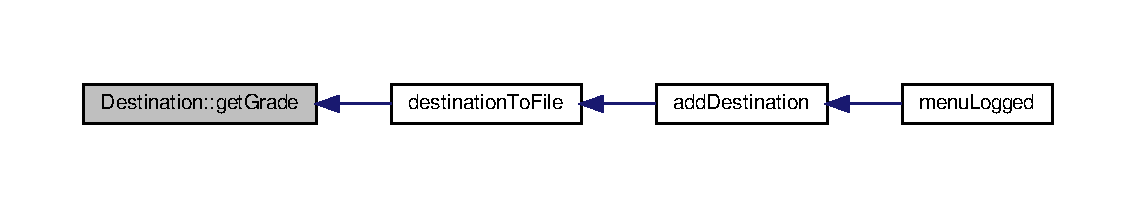
\includegraphics[width=350pt]{class_destination_a34dd7a2072743078d5067d336dc3c25d_icgraph}
\end{center}
\end{figure}
\mbox{\Hypertarget{class_destination_ade746815624a6fd5add31a3475e04b45}\label{class_destination_ade746815624a6fd5add31a3475e04b45}} 
\index{Destination@{Destination}!get\+Photos@{get\+Photos}}
\index{get\+Photos@{get\+Photos}!Destination@{Destination}}
\subsubsection{\texorpdfstring{get\+Photos()}{getPhotos()}}
{\footnotesize\ttfamily vector$<$string$>$ Destination\+::get\+Photos (\begin{DoxyParamCaption}{ }\end{DoxyParamCaption}) const\hspace{0.3cm}{\ttfamily [inline]}}

Getter for photos. \begin{DoxyReturn}{Returns}
vector$<$string$>$ photos 
\end{DoxyReturn}
Here is the caller graph for this function\+:\nopagebreak
\begin{figure}[H]
\begin{center}
\leavevmode
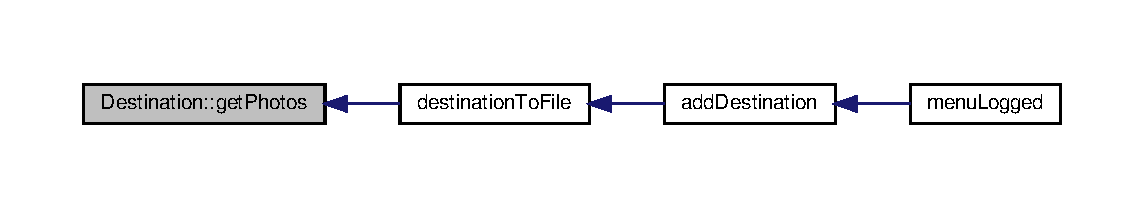
\includegraphics[width=350pt]{class_destination_ade746815624a6fd5add31a3475e04b45_icgraph}
\end{center}
\end{figure}
\mbox{\Hypertarget{class_destination_a6a98c7e1c0ffa4b821d3f7dd85cad3dd}\label{class_destination_a6a98c7e1c0ffa4b821d3f7dd85cad3dd}} 
\index{Destination@{Destination}!get\+To\+Date@{get\+To\+Date}}
\index{get\+To\+Date@{get\+To\+Date}!Destination@{Destination}}
\subsubsection{\texorpdfstring{get\+To\+Date()}{getToDate()}}
{\footnotesize\ttfamily \hyperlink{class_date}{Date} Destination\+::get\+To\+Date (\begin{DoxyParamCaption}{ }\end{DoxyParamCaption}) const\hspace{0.3cm}{\ttfamily [inline]}}

Getter for end date. \begin{DoxyReturn}{Returns}
\hyperlink{class_date}{Date} to 
\end{DoxyReturn}
Here is the caller graph for this function\+:\nopagebreak
\begin{figure}[H]
\begin{center}
\leavevmode
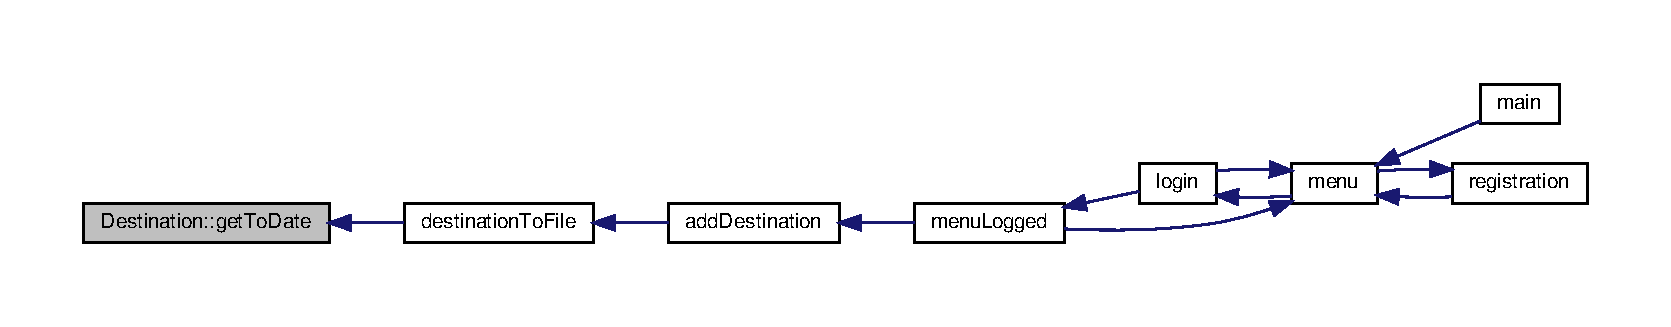
\includegraphics[width=350pt]{class_destination_a6a98c7e1c0ffa4b821d3f7dd85cad3dd_icgraph}
\end{center}
\end{figure}
\mbox{\Hypertarget{class_destination_a08199ade6e0bf7488d796d85dec8cfd9}\label{class_destination_a08199ade6e0bf7488d796d85dec8cfd9}} 
\index{Destination@{Destination}!set\+Comment@{set\+Comment}}
\index{set\+Comment@{set\+Comment}!Destination@{Destination}}
\subsubsection{\texorpdfstring{set\+Comment()}{setComment()}}
{\footnotesize\ttfamily void Destination\+::set\+Comment (\begin{DoxyParamCaption}\item[{string}]{comm }\end{DoxyParamCaption})}

Method setting the comment. Here is the caller graph for this function\+:\nopagebreak
\begin{figure}[H]
\begin{center}
\leavevmode
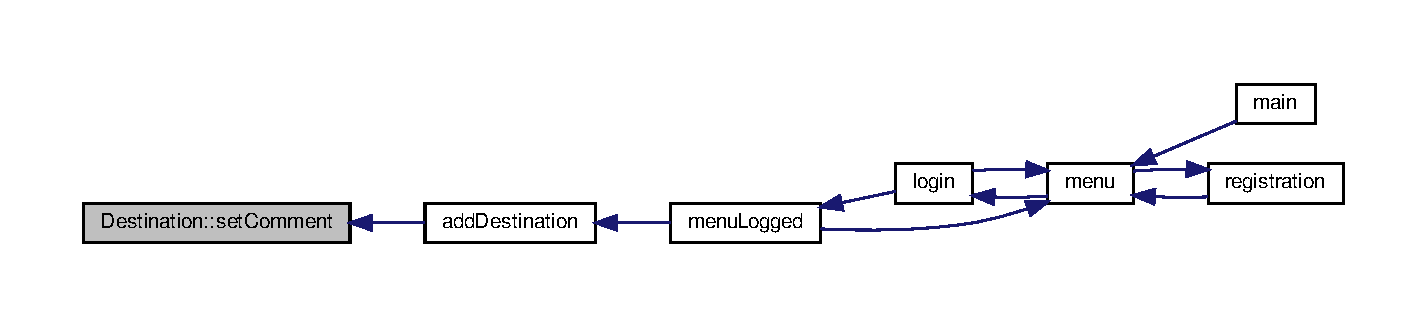
\includegraphics[width=350pt]{class_destination_a08199ade6e0bf7488d796d85dec8cfd9_icgraph}
\end{center}
\end{figure}
\mbox{\Hypertarget{class_destination_a9cafaaf83be9ea548401caf2a2c4d839}\label{class_destination_a9cafaaf83be9ea548401caf2a2c4d839}} 
\index{Destination@{Destination}!set\+Destination@{set\+Destination}}
\index{set\+Destination@{set\+Destination}!Destination@{Destination}}
\subsubsection{\texorpdfstring{set\+Destination()}{setDestination()}}
{\footnotesize\ttfamily void Destination\+::set\+Destination (\begin{DoxyParamCaption}\item[{string}]{dest }\end{DoxyParamCaption})}

Methood setting the destination(location). Here is the caller graph for this function\+:\nopagebreak
\begin{figure}[H]
\begin{center}
\leavevmode
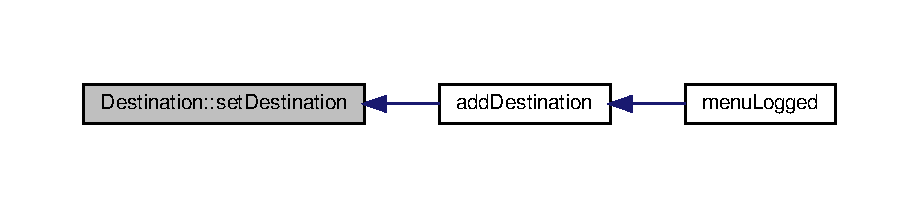
\includegraphics[width=350pt]{class_destination_a9cafaaf83be9ea548401caf2a2c4d839_icgraph}
\end{center}
\end{figure}
\mbox{\Hypertarget{class_destination_a6fc539f51a5fd6844fef290facc4e887}\label{class_destination_a6fc539f51a5fd6844fef290facc4e887}} 
\index{Destination@{Destination}!set\+From\+Date@{set\+From\+Date}}
\index{set\+From\+Date@{set\+From\+Date}!Destination@{Destination}}
\subsubsection{\texorpdfstring{set\+From\+Date()}{setFromDate()}}
{\footnotesize\ttfamily void Destination\+::set\+From\+Date (\begin{DoxyParamCaption}\item[{\hyperlink{class_date}{Date}}]{fr }\end{DoxyParamCaption})}

Method setting the start date. Here is the caller graph for this function\+:\nopagebreak
\begin{figure}[H]
\begin{center}
\leavevmode
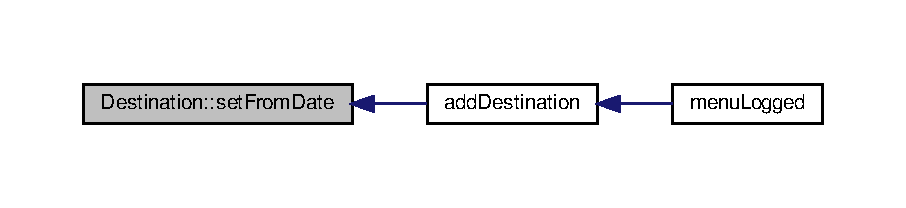
\includegraphics[width=350pt]{class_destination_a6fc539f51a5fd6844fef290facc4e887_icgraph}
\end{center}
\end{figure}
\mbox{\Hypertarget{class_destination_ac7f1c3be54b5223aa1e9ad4523ef6976}\label{class_destination_ac7f1c3be54b5223aa1e9ad4523ef6976}} 
\index{Destination@{Destination}!set\+Grade@{set\+Grade}}
\index{set\+Grade@{set\+Grade}!Destination@{Destination}}
\subsubsection{\texorpdfstring{set\+Grade()}{setGrade()}}
{\footnotesize\ttfamily void Destination\+::set\+Grade (\begin{DoxyParamCaption}\item[{unsigned}]{gr }\end{DoxyParamCaption})}

Method setting the grade. Here is the caller graph for this function\+:\nopagebreak
\begin{figure}[H]
\begin{center}
\leavevmode
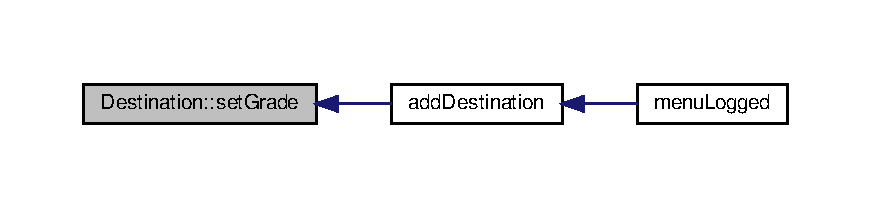
\includegraphics[width=350pt]{class_destination_ac7f1c3be54b5223aa1e9ad4523ef6976_icgraph}
\end{center}
\end{figure}
\mbox{\Hypertarget{class_destination_afec038764d48882a9005cea50e418219}\label{class_destination_afec038764d48882a9005cea50e418219}} 
\index{Destination@{Destination}!set\+To\+Date@{set\+To\+Date}}
\index{set\+To\+Date@{set\+To\+Date}!Destination@{Destination}}
\subsubsection{\texorpdfstring{set\+To\+Date()}{setToDate()}}
{\footnotesize\ttfamily void Destination\+::set\+To\+Date (\begin{DoxyParamCaption}\item[{\hyperlink{class_date}{Date}}]{t }\end{DoxyParamCaption})}

Method setting the end date. Here is the caller graph for this function\+:\nopagebreak
\begin{figure}[H]
\begin{center}
\leavevmode
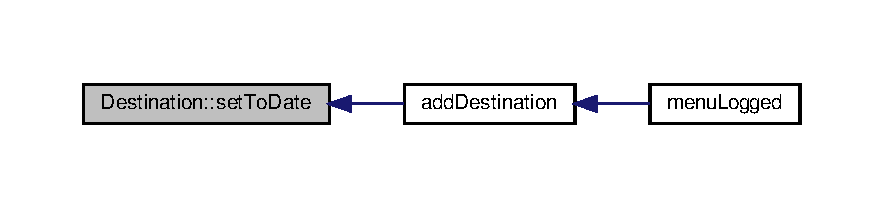
\includegraphics[width=350pt]{class_destination_afec038764d48882a9005cea50e418219_icgraph}
\end{center}
\end{figure}


\subsection{Member Data Documentation}
\mbox{\Hypertarget{class_destination_a4788b97b93c5336a8717540e0daa841a}\label{class_destination_a4788b97b93c5336a8717540e0daa841a}} 
\index{Destination@{Destination}!comment@{comment}}
\index{comment@{comment}!Destination@{Destination}}
\subsubsection{\texorpdfstring{comment}{comment}}
{\footnotesize\ttfamily string Destination\+::comment\hspace{0.3cm}{\ttfamily [private]}}

Variable for comment. \mbox{\Hypertarget{class_destination_ad5bc042020c7faf68d8940061142a0ea}\label{class_destination_ad5bc042020c7faf68d8940061142a0ea}} 
\index{Destination@{Destination}!destination@{destination}}
\index{destination@{destination}!Destination@{Destination}}
\subsubsection{\texorpdfstring{destination}{destination}}
{\footnotesize\ttfamily string Destination\+::destination\hspace{0.3cm}{\ttfamily [private]}}

Variable for destination(location). \mbox{\Hypertarget{class_destination_a0dea129cf2457e922c57b7fb5996509a}\label{class_destination_a0dea129cf2457e922c57b7fb5996509a}} 
\index{Destination@{Destination}!from@{from}}
\index{from@{from}!Destination@{Destination}}
\subsubsection{\texorpdfstring{from}{from}}
{\footnotesize\ttfamily \hyperlink{class_date}{Date} Destination\+::from\hspace{0.3cm}{\ttfamily [private]}}

Variable for start date. \mbox{\Hypertarget{class_destination_afbab7d354ba8c639501755e48261012e}\label{class_destination_afbab7d354ba8c639501755e48261012e}} 
\index{Destination@{Destination}!grade@{grade}}
\index{grade@{grade}!Destination@{Destination}}
\subsubsection{\texorpdfstring{grade}{grade}}
{\footnotesize\ttfamily unsigned Destination\+::grade\hspace{0.3cm}{\ttfamily [private]}}

Variable for grade. \mbox{\Hypertarget{class_destination_a17cb8de845ce9d65eb7082c79c617444}\label{class_destination_a17cb8de845ce9d65eb7082c79c617444}} 
\index{Destination@{Destination}!photos@{photos}}
\index{photos@{photos}!Destination@{Destination}}
\subsubsection{\texorpdfstring{photos}{photos}}
{\footnotesize\ttfamily vector$<$string$>$ Destination\+::photos\hspace{0.3cm}{\ttfamily [private]}}

Variable for photos. \mbox{\Hypertarget{class_destination_ad556f5592b3bcb4ab407064bc1f0763c}\label{class_destination_ad556f5592b3bcb4ab407064bc1f0763c}} 
\index{Destination@{Destination}!to@{to}}
\index{to@{to}!Destination@{Destination}}
\subsubsection{\texorpdfstring{to}{to}}
{\footnotesize\ttfamily \hyperlink{class_date}{Date} Destination\+::to\hspace{0.3cm}{\ttfamily [private]}}

Variable for end date. 

The documentation for this class was generated from the following files\+:\begin{DoxyCompactItemize}
\item 
\hyperlink{destination_8h}{destination.\+h}\item 
\hyperlink{destination_8cpp}{destination.\+cpp}\end{DoxyCompactItemize}

\hypertarget{class_user}{}\section{User Class Reference}
\label{class_user}\index{User@{User}}


A user class.  




{\ttfamily \#include $<$user.\+h$>$}

\subsection*{Public Member Functions}
\begin{DoxyCompactItemize}
\item 
\hyperlink{class_user_acefd113882ab5f80ea087401b7f9d0b4}{User} (const string \&=\char`\"{}\char`\"{}, const string \&=\char`\"{}\char`\"{}, const string \&=\char`\"{}\char`\"{}, int=0)
\item 
\hyperlink{class_user_aad23b10cdefd26d6ca2ca981e9f9c973}{User} (const \hyperlink{class_user}{User} \&other)
\item 
\hyperlink{class_user}{User} \& \hyperlink{class_user_a00fe82353b0ee8cf6abb1088d36e125b}{operator=} (const \hyperlink{class_user}{User} \&other)
\item 
void \hyperlink{class_user_a453323a9766e086f1967a96d79fc8b76}{set\+Username} (string)
\item 
void \hyperlink{class_user_ab8d3c965902b378fc3472b388a97d56d}{set\+Password} (string)
\item 
void \hyperlink{class_user_a79486f90c900c5dfc272f0ad9a204c95}{set\+Email} (string)
\item 
string \hyperlink{class_user_a82e034043e04b2d750c654c8b2f2ce78}{get\+Username} () const
\item 
string \hyperlink{class_user_a33429bdd1253091697a9c5c5e1448bee}{get\+Password} () const
\item 
string \hyperlink{class_user_a4c647e583bd964f40f687776a0d185dc}{get\+Email} () const
\end{DoxyCompactItemize}
\subsection*{Friends}
\begin{DoxyCompactItemize}
\item 
ostream \& \hyperlink{class_user_acf1038a8d320684dc3fbdd5e4308e062}{operator$<$$<$} (ostream \&out, const \hyperlink{class_user}{User} \&user)
\item 
istream \& \hyperlink{class_user_aae624f64cdd1af3b59c2443cffa82494}{operator$>$$>$} (istream \&in, \hyperlink{class_user}{User} \&user)
\end{DoxyCompactItemize}


\subsection{Detailed Description}
A user class. 

This class is used to initialize a user. The user is the main structure part of the project. Every creation of a profile is initializing a new \hyperlink{class_user}{User}. In order to log in you need to access a \hyperlink{class_user}{User}. 

\subsection{Constructor \& Destructor Documentation}
\mbox{\Hypertarget{class_user_acefd113882ab5f80ea087401b7f9d0b4}\label{class_user_acefd113882ab5f80ea087401b7f9d0b4}} 
\index{User@{User}!User@{User}}
\index{User@{User}!User@{User}}
\subsubsection{\texorpdfstring{User()}{User()}\hspace{0.1cm}{\footnotesize\ttfamily [1/2]}}
{\footnotesize\ttfamily User\+::\+User (\begin{DoxyParamCaption}\item[{const string \&}]{un = {\ttfamily \char`\"{}\char`\"{}},  }\item[{const string \&}]{pass = {\ttfamily \char`\"{}\char`\"{}},  }\item[{const string \&}]{em = {\ttfamily \char`\"{}\char`\"{}},  }\item[{int}]{num\+Des = {\ttfamily 0} }\end{DoxyParamCaption})}

A parametrized constructor with default vlaues. \mbox{\Hypertarget{class_user_aad23b10cdefd26d6ca2ca981e9f9c973}\label{class_user_aad23b10cdefd26d6ca2ca981e9f9c973}} 
\index{User@{User}!User@{User}}
\index{User@{User}!User@{User}}
\subsubsection{\texorpdfstring{User()}{User()}\hspace{0.1cm}{\footnotesize\ttfamily [2/2]}}
{\footnotesize\ttfamily User\+::\+User (\begin{DoxyParamCaption}\item[{const \hyperlink{class_user}{User} \&}]{other }\end{DoxyParamCaption})}

A copy constructor. 

\subsection{Member Function Documentation}
\mbox{\Hypertarget{class_user_a4c647e583bd964f40f687776a0d185dc}\label{class_user_a4c647e583bd964f40f687776a0d185dc}} 
\index{User@{User}!get\+Email@{get\+Email}}
\index{get\+Email@{get\+Email}!User@{User}}
\subsubsection{\texorpdfstring{get\+Email()}{getEmail()}}
{\footnotesize\ttfamily string User\+::get\+Email (\begin{DoxyParamCaption}{ }\end{DoxyParamCaption}) const\hspace{0.3cm}{\ttfamily [inline]}}

Getter for email. \begin{DoxyReturn}{Returns}
string email 
\end{DoxyReturn}
Here is the caller graph for this function\+:\nopagebreak
\begin{figure}[H]
\begin{center}
\leavevmode
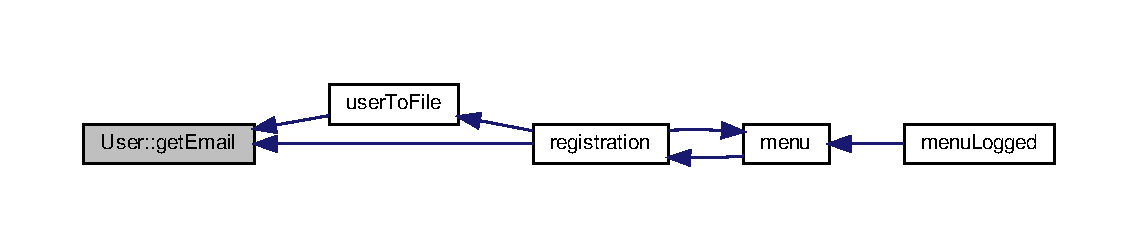
\includegraphics[width=350pt]{class_user_a4c647e583bd964f40f687776a0d185dc_icgraph}
\end{center}
\end{figure}
\mbox{\Hypertarget{class_user_a33429bdd1253091697a9c5c5e1448bee}\label{class_user_a33429bdd1253091697a9c5c5e1448bee}} 
\index{User@{User}!get\+Password@{get\+Password}}
\index{get\+Password@{get\+Password}!User@{User}}
\subsubsection{\texorpdfstring{get\+Password()}{getPassword()}}
{\footnotesize\ttfamily string User\+::get\+Password (\begin{DoxyParamCaption}{ }\end{DoxyParamCaption}) const\hspace{0.3cm}{\ttfamily [inline]}}

Getter for password. \begin{DoxyReturn}{Returns}
string password 
\end{DoxyReturn}
Here is the caller graph for this function\+:\nopagebreak
\begin{figure}[H]
\begin{center}
\leavevmode
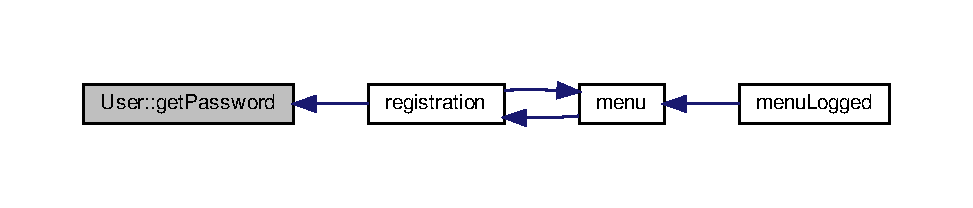
\includegraphics[width=350pt]{class_user_a33429bdd1253091697a9c5c5e1448bee_icgraph}
\end{center}
\end{figure}
\mbox{\Hypertarget{class_user_a82e034043e04b2d750c654c8b2f2ce78}\label{class_user_a82e034043e04b2d750c654c8b2f2ce78}} 
\index{User@{User}!get\+Username@{get\+Username}}
\index{get\+Username@{get\+Username}!User@{User}}
\subsubsection{\texorpdfstring{get\+Username()}{getUsername()}}
{\footnotesize\ttfamily string User\+::get\+Username (\begin{DoxyParamCaption}{ }\end{DoxyParamCaption}) const\hspace{0.3cm}{\ttfamily [inline]}}

Getter for username. \begin{DoxyReturn}{Returns}
string username 
\end{DoxyReturn}
Here is the caller graph for this function\+:\nopagebreak
\begin{figure}[H]
\begin{center}
\leavevmode
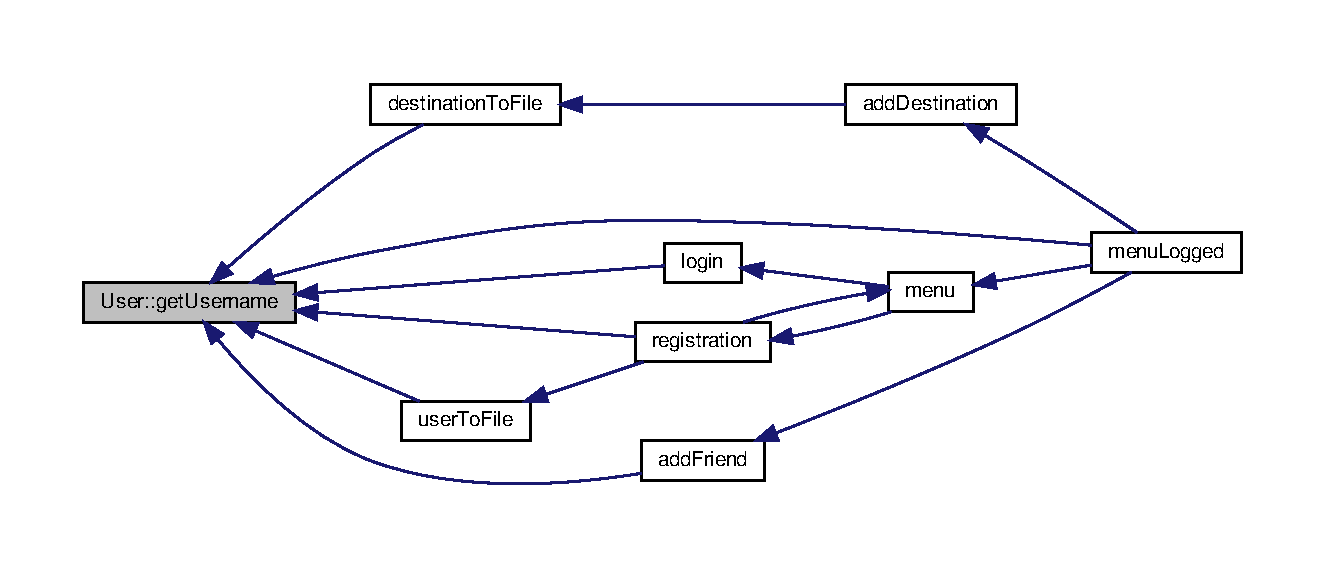
\includegraphics[width=350pt]{class_user_a82e034043e04b2d750c654c8b2f2ce78_icgraph}
\end{center}
\end{figure}
\mbox{\Hypertarget{class_user_a00fe82353b0ee8cf6abb1088d36e125b}\label{class_user_a00fe82353b0ee8cf6abb1088d36e125b}} 
\index{User@{User}!operator=@{operator=}}
\index{operator=@{operator=}!User@{User}}
\subsubsection{\texorpdfstring{operator=()}{operator=()}}
{\footnotesize\ttfamily \hyperlink{class_user}{User} \& User\+::operator= (\begin{DoxyParamCaption}\item[{const \hyperlink{class_user}{User} \&}]{other }\end{DoxyParamCaption})}

Operator=. \mbox{\Hypertarget{class_user_a79486f90c900c5dfc272f0ad9a204c95}\label{class_user_a79486f90c900c5dfc272f0ad9a204c95}} 
\index{User@{User}!set\+Email@{set\+Email}}
\index{set\+Email@{set\+Email}!User@{User}}
\subsubsection{\texorpdfstring{set\+Email()}{setEmail()}}
{\footnotesize\ttfamily void User\+::set\+Email (\begin{DoxyParamCaption}\item[{string}]{em }\end{DoxyParamCaption})}

Method setting the email. Here is the caller graph for this function\+:\nopagebreak
\begin{figure}[H]
\begin{center}
\leavevmode
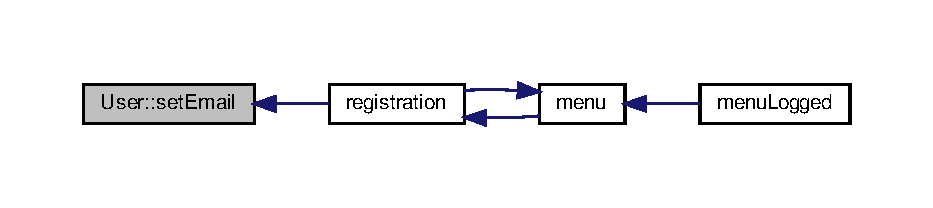
\includegraphics[width=350pt]{class_user_a79486f90c900c5dfc272f0ad9a204c95_icgraph}
\end{center}
\end{figure}
\mbox{\Hypertarget{class_user_ab8d3c965902b378fc3472b388a97d56d}\label{class_user_ab8d3c965902b378fc3472b388a97d56d}} 
\index{User@{User}!set\+Password@{set\+Password}}
\index{set\+Password@{set\+Password}!User@{User}}
\subsubsection{\texorpdfstring{set\+Password()}{setPassword()}}
{\footnotesize\ttfamily void User\+::set\+Password (\begin{DoxyParamCaption}\item[{string}]{pass }\end{DoxyParamCaption})}

Method setting the password. Here is the caller graph for this function\+:\nopagebreak
\begin{figure}[H]
\begin{center}
\leavevmode
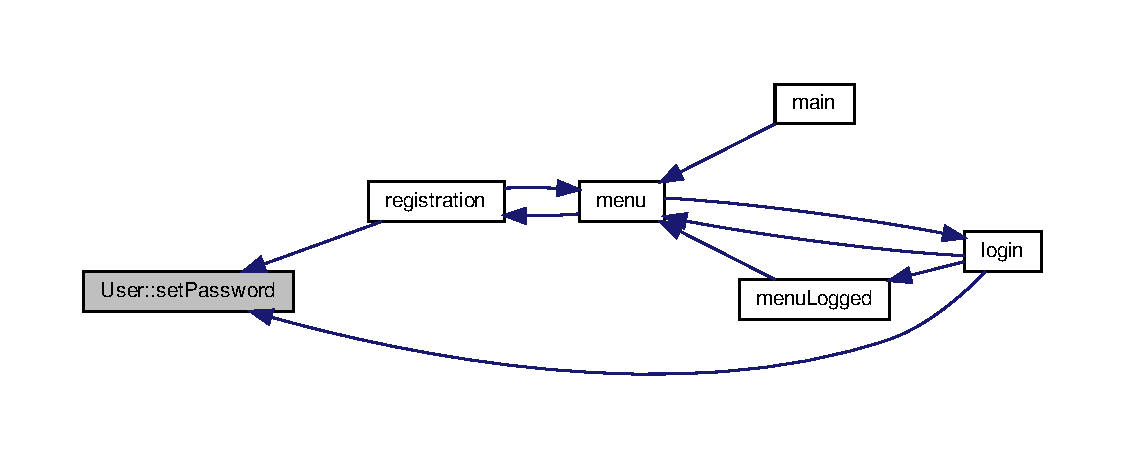
\includegraphics[width=350pt]{class_user_ab8d3c965902b378fc3472b388a97d56d_icgraph}
\end{center}
\end{figure}
\mbox{\Hypertarget{class_user_a453323a9766e086f1967a96d79fc8b76}\label{class_user_a453323a9766e086f1967a96d79fc8b76}} 
\index{User@{User}!set\+Username@{set\+Username}}
\index{set\+Username@{set\+Username}!User@{User}}
\subsubsection{\texorpdfstring{set\+Username()}{setUsername()}}
{\footnotesize\ttfamily void User\+::set\+Username (\begin{DoxyParamCaption}\item[{string}]{un }\end{DoxyParamCaption})}

Method setting the username. Here is the caller graph for this function\+:\nopagebreak
\begin{figure}[H]
\begin{center}
\leavevmode
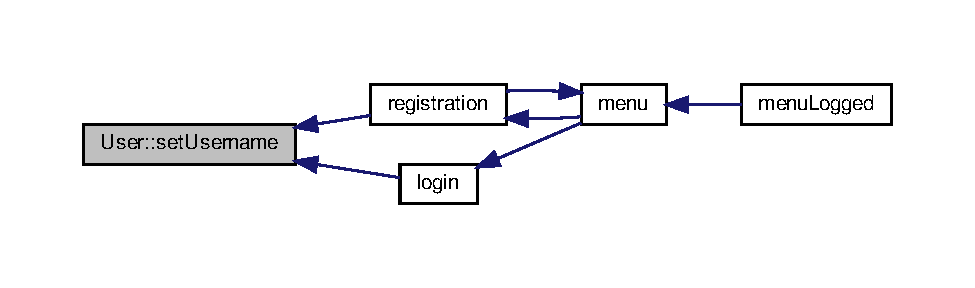
\includegraphics[width=350pt]{class_user_a453323a9766e086f1967a96d79fc8b76_icgraph}
\end{center}
\end{figure}


\subsection{Friends And Related Function Documentation}
\mbox{\Hypertarget{class_user_acf1038a8d320684dc3fbdd5e4308e062}\label{class_user_acf1038a8d320684dc3fbdd5e4308e062}} 
\index{User@{User}!operator$<$$<$@{operator$<$$<$}}
\index{operator$<$$<$@{operator$<$$<$}!User@{User}}
\subsubsection{\texorpdfstring{operator$<$$<$}{operator<<}}
{\footnotesize\ttfamily ostream\& operator$<$$<$ (\begin{DoxyParamCaption}\item[{ostream \&}]{out,  }\item[{const \hyperlink{class_user}{User} \&}]{user }\end{DoxyParamCaption})\hspace{0.3cm}{\ttfamily [friend]}}

Overloaded operator$<$$<$. \mbox{\Hypertarget{class_user_aae624f64cdd1af3b59c2443cffa82494}\label{class_user_aae624f64cdd1af3b59c2443cffa82494}} 
\index{User@{User}!operator$>$$>$@{operator$>$$>$}}
\index{operator$>$$>$@{operator$>$$>$}!User@{User}}
\subsubsection{\texorpdfstring{operator$>$$>$}{operator>>}}
{\footnotesize\ttfamily istream\& operator$>$$>$ (\begin{DoxyParamCaption}\item[{istream \&}]{in,  }\item[{\hyperlink{class_user}{User} \&}]{user }\end{DoxyParamCaption})\hspace{0.3cm}{\ttfamily [friend]}}

Overloaded operator$>$$>$. 

The documentation for this class was generated from the following files\+:\begin{DoxyCompactItemize}
\item 
user.\+h\item 
user.\+cpp\end{DoxyCompactItemize}

\chapter{File Documentation}
\hypertarget{application_8h}{}\section{application.\+h File Reference}
\label{application_8h}\index{application.\+h@{application.\+h}}
{\ttfamily \#include $<$iostream$>$}\newline
{\ttfamily \#include $<$fstream$>$}\newline
{\ttfamily \#include $<$string$>$}\newline
{\ttfamily \#include $<$cstdlib$>$}\newline
{\ttfamily \#include \char`\"{}user.\+h\char`\"{}}\newline
{\ttfamily \#include \char`\"{}destination.\+h\char`\"{}}\newline
{\ttfamily \#include \char`\"{}date.\+h\char`\"{}}\newline
{\ttfamily \#include \char`\"{}read\+File.\+h\char`\"{}}\newline
Include dependency graph for application.\+h\+:\nopagebreak
\begin{figure}[H]
\begin{center}
\leavevmode
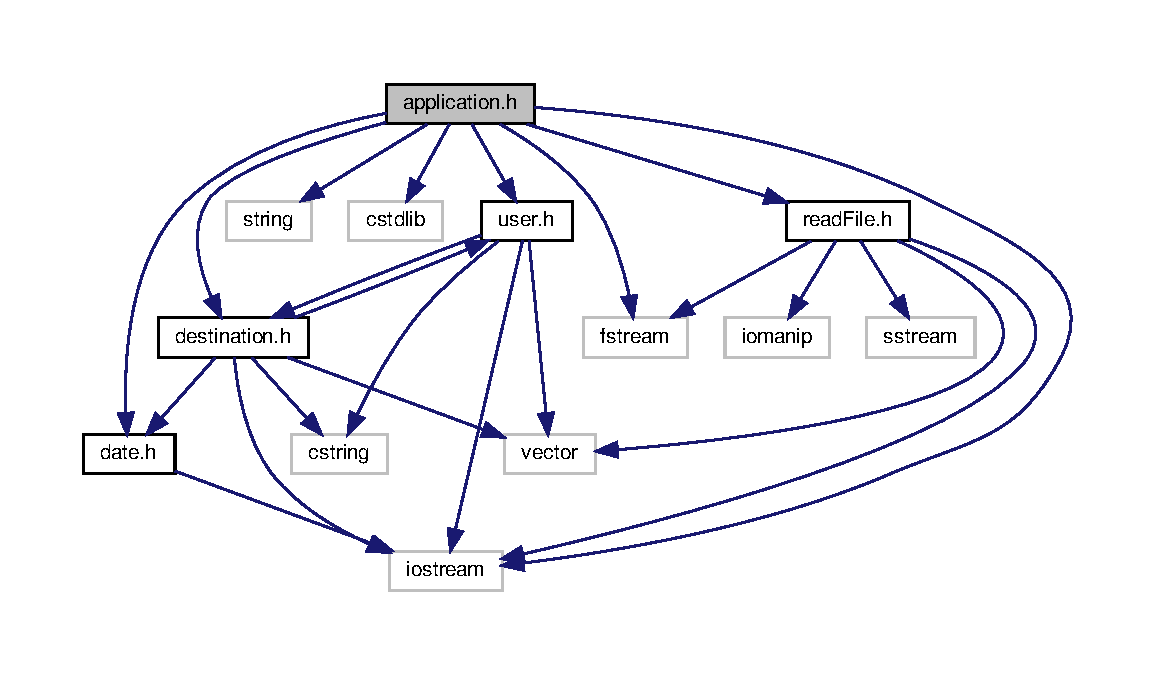
\includegraphics[width=350pt]{application_8h__incl}
\end{center}
\end{figure}
This graph shows which files directly or indirectly include this file\+:\nopagebreak
\begin{figure}[H]
\begin{center}
\leavevmode
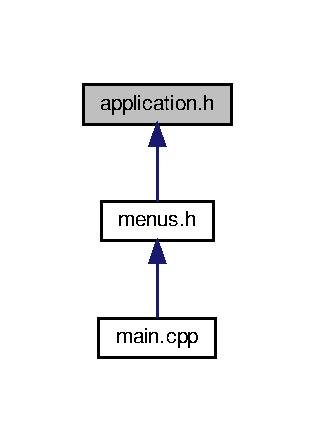
\includegraphics[width=151pt]{application_8h__dep__incl}
\end{center}
\end{figure}
\subsection*{Functions}
\begin{DoxyCompactItemize}
\item 
void \hyperlink{application_8h_acc3ffb5f9c459368ca3ca9815d499af2}{add\+Destination} (const \hyperlink{class_user}{User} \&)
\item 
void \hyperlink{application_8h_a92aba65fab778922f928e9d9bf6475d6}{add\+Friend} (const \hyperlink{class_user}{User} \&)
\item 
void \hyperlink{application_8h_a3ca98c5244a06fb6199d64f44b6a2fa4}{destination\+To\+File} (const \hyperlink{class_user}{User} \&, const \hyperlink{class_destination}{Destination} \&, int)
\item 
void \hyperlink{application_8h_adf656ece2632a1013b0e510fbb0ac529}{user\+To\+File} (const \hyperlink{class_user}{User} \&being\+Reg)
\item 
string \hyperlink{application_8h_a265d79751fc2100c17b58f15df75fed8}{add\+Location} ()
\item 
\hyperlink{class_date}{Date} \hyperlink{application_8h_a9066e8999df2f39d7ffeb81176fb14d4}{add\+Start\+Date} ()
\item 
\hyperlink{class_date}{Date} \hyperlink{application_8h_a6a7fe6d7e0e844cb0d599228c331b2a1}{add\+End\+Date} ()
\item 
unsigned \hyperlink{application_8h_a58f4936001855f43fb36be2c1dda8542}{add\+Grade} ()
\item 
string \hyperlink{application_8h_abd4c9e6dd42fc406bcd9eb172027f30e}{add\+Comment} ()
\item 
vector$<$ string $>$ \hyperlink{application_8h_a3fd32a66da2ec32c0823ad407e7d1f62}{add\+Photos} (int)
\item 
\mbox{\Hypertarget{application_8h_a2846723ff3141f7044bf9cfa3514fce9}\label{application_8h_a2846723ff3141f7044bf9cfa3514fce9}} 
void {\bfseries copy\+File\+To\+Another\+File} ()
\item 
\mbox{\Hypertarget{application_8h_a56b247a576ce83fffe54cb75d85f1538}\label{application_8h_a56b247a576ce83fffe54cb75d85f1538}} 
void {\bfseries string\+To\+Users\+DB} (const matrix \&users\+File, const \hyperlink{class_user}{User} \&logged\+In\+User, const string \&friend\+To\+Be\+Added)
\end{DoxyCompactItemize}


\subsection{Function Documentation}
\mbox{\Hypertarget{application_8h_abd4c9e6dd42fc406bcd9eb172027f30e}\label{application_8h_abd4c9e6dd42fc406bcd9eb172027f30e}} 
\index{application.\+h@{application.\+h}!add\+Comment@{add\+Comment}}
\index{add\+Comment@{add\+Comment}!application.\+h@{application.\+h}}
\subsubsection{\texorpdfstring{add\+Comment()}{addComment()}}
{\footnotesize\ttfamily string add\+Comment (\begin{DoxyParamCaption}{ }\end{DoxyParamCaption})}

This fucntion is asking the user to input a comment about the trip. \begin{DoxyReturn}{Returns}
string(comment) 
\end{DoxyReturn}
Here is the caller graph for this function\+:\nopagebreak
\begin{figure}[H]
\begin{center}
\leavevmode
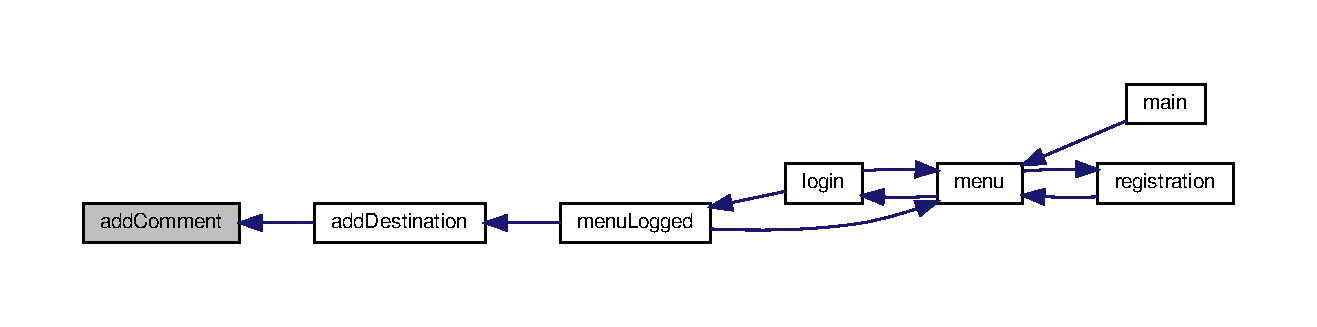
\includegraphics[width=350pt]{application_8h_abd4c9e6dd42fc406bcd9eb172027f30e_icgraph}
\end{center}
\end{figure}
\mbox{\Hypertarget{application_8h_acc3ffb5f9c459368ca3ca9815d499af2}\label{application_8h_acc3ffb5f9c459368ca3ca9815d499af2}} 
\index{application.\+h@{application.\+h}!add\+Destination@{add\+Destination}}
\index{add\+Destination@{add\+Destination}!application.\+h@{application.\+h}}
\subsubsection{\texorpdfstring{add\+Destination()}{addDestination()}}
{\footnotesize\ttfamily void add\+Destination (\begin{DoxyParamCaption}\item[{const \hyperlink{class_user}{User} \&}]{logged\+In\+User }\end{DoxyParamCaption})}

This function is accepting an object of type \hyperlink{class_user}{User} and is used to add a trip(destination) to the \hyperlink{class_user}{User}\textquotesingle{}s database. Firstly, the function initialize an \char`\"{}empty\char`\"{} destination and uses other functions and the setters of class \hyperlink{class_destination}{Destination} to set location, period, grade, comment and photos to the location. 
\begin{DoxyParams}{Parameters}
{\em const} & \hyperlink{class_user}{User}\& logged\+In\+User \\
\hline
\end{DoxyParams}
Here is the call graph for this function\+:\nopagebreak
\begin{figure}[H]
\begin{center}
\leavevmode
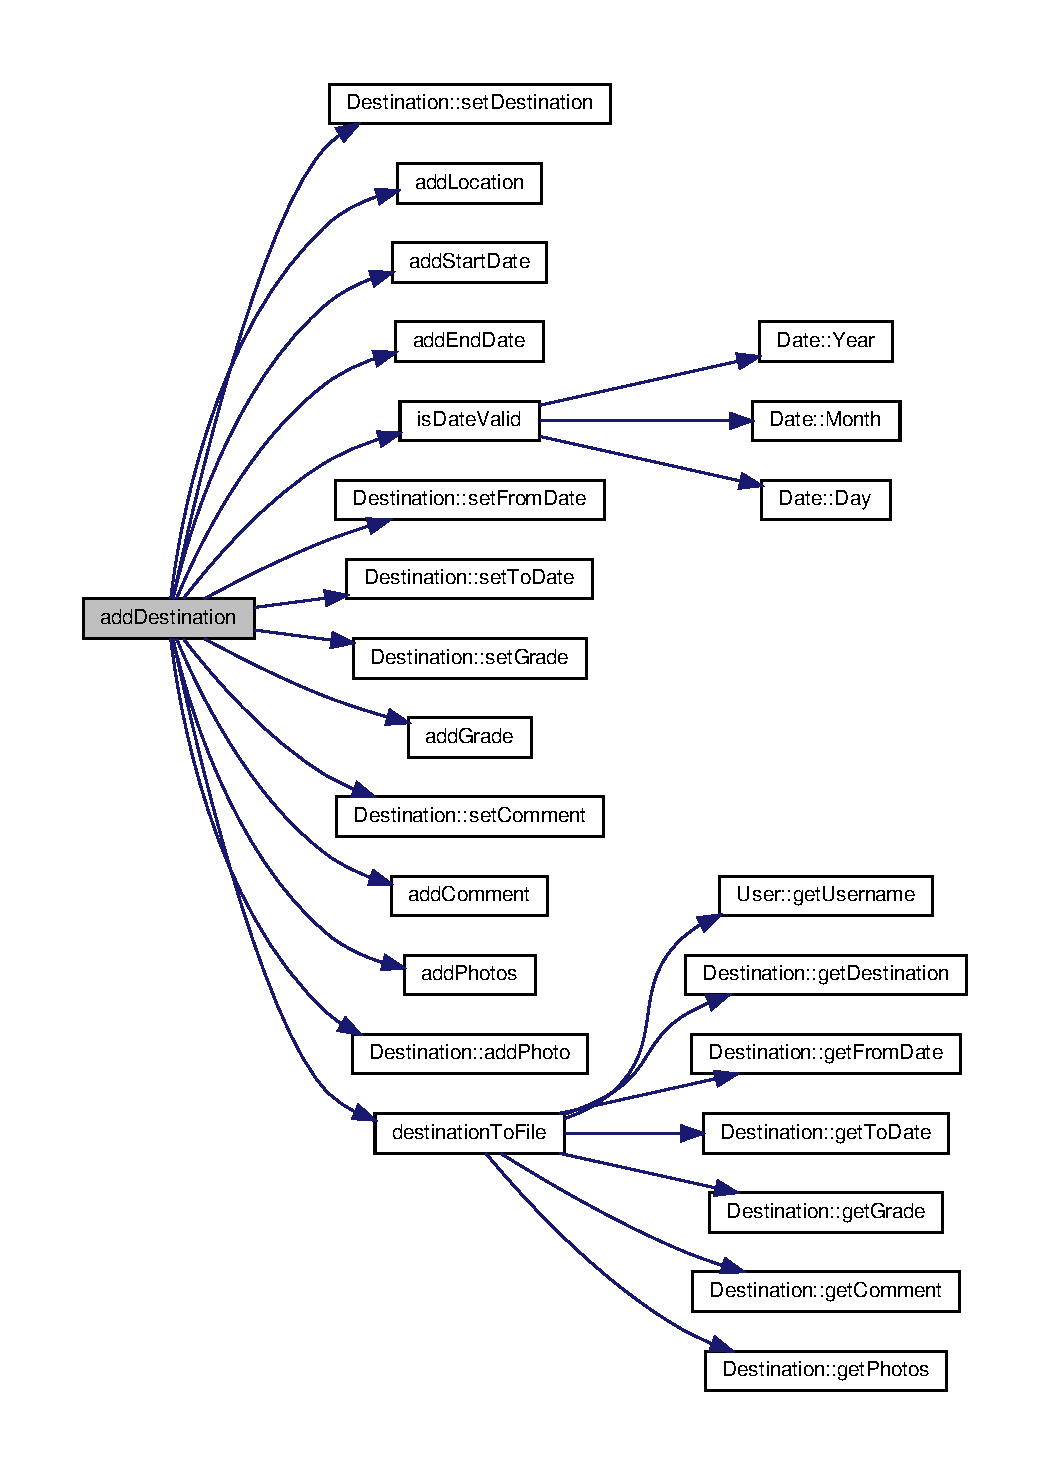
\includegraphics[width=350pt]{application_8h_acc3ffb5f9c459368ca3ca9815d499af2_cgraph}
\end{center}
\end{figure}
Here is the caller graph for this function\+:\nopagebreak
\begin{figure}[H]
\begin{center}
\leavevmode
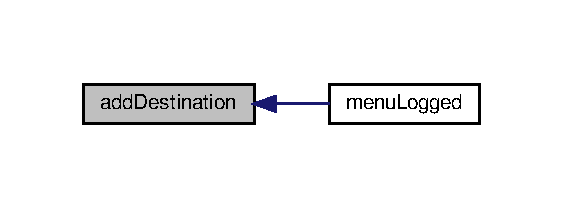
\includegraphics[width=270pt]{application_8h_acc3ffb5f9c459368ca3ca9815d499af2_icgraph}
\end{center}
\end{figure}
\mbox{\Hypertarget{application_8h_a6a7fe6d7e0e844cb0d599228c331b2a1}\label{application_8h_a6a7fe6d7e0e844cb0d599228c331b2a1}} 
\index{application.\+h@{application.\+h}!add\+End\+Date@{add\+End\+Date}}
\index{add\+End\+Date@{add\+End\+Date}!application.\+h@{application.\+h}}
\subsubsection{\texorpdfstring{add\+End\+Date()}{addEndDate()}}
{\footnotesize\ttfamily \hyperlink{class_date}{Date} add\+End\+Date (\begin{DoxyParamCaption}{ }\end{DoxyParamCaption})}

This function is asking the user to input the end date and is initializing an object of type \hyperlink{class_date}{Date}. \begin{DoxyReturn}{Returns}
\hyperlink{class_date}{Date(end date)} 
\end{DoxyReturn}
Here is the caller graph for this function\+:\nopagebreak
\begin{figure}[H]
\begin{center}
\leavevmode
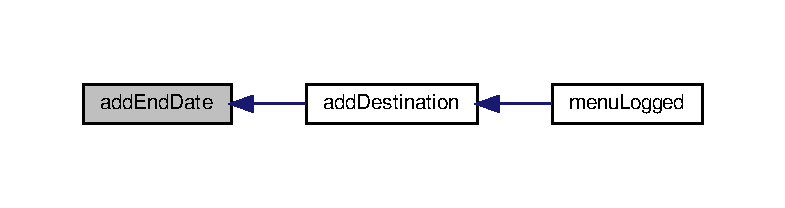
\includegraphics[width=350pt]{application_8h_a6a7fe6d7e0e844cb0d599228c331b2a1_icgraph}
\end{center}
\end{figure}
\mbox{\Hypertarget{application_8h_a92aba65fab778922f928e9d9bf6475d6}\label{application_8h_a92aba65fab778922f928e9d9bf6475d6}} 
\index{application.\+h@{application.\+h}!add\+Friend@{add\+Friend}}
\index{add\+Friend@{add\+Friend}!application.\+h@{application.\+h}}
\subsubsection{\texorpdfstring{add\+Friend()}{addFriend()}}
{\footnotesize\ttfamily void add\+Friend (\begin{DoxyParamCaption}\item[{const \hyperlink{class_user}{User} \&}]{logged\+In\+User }\end{DoxyParamCaption})}

The function accepts an object of type \hyperlink{class_user}{User} and is adding another \hyperlink{class_user}{User}\textquotesingle{}s username in the friend list of the accepted object. Some vertifications are made. Firstly, whether such a username exists in the database. Secondly, ensuring that the user is not trying to add himself as friend. Then checking whether the inputted username is already in the friend list. 
\begin{DoxyParams}{Parameters}
{\em const} & \hyperlink{class_user}{User}\& logged\+In\+User \\
\hline
\end{DoxyParams}
Here is the call graph for this function\+:\nopagebreak
\begin{figure}[H]
\begin{center}
\leavevmode
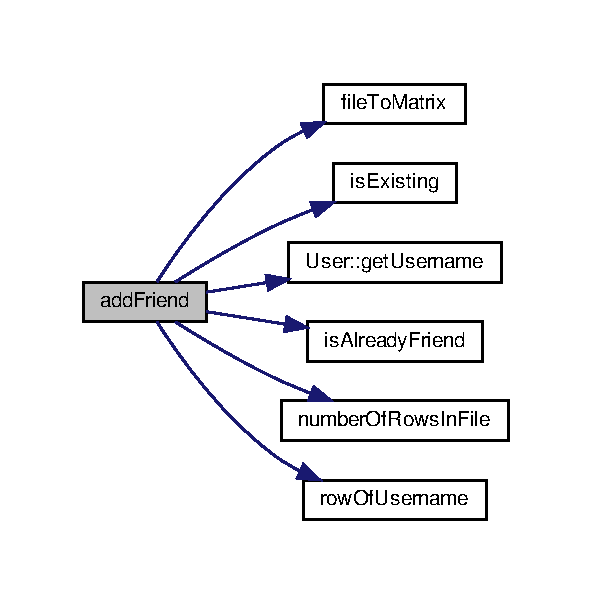
\includegraphics[width=277pt]{application_8h_a92aba65fab778922f928e9d9bf6475d6_cgraph}
\end{center}
\end{figure}
Here is the caller graph for this function\+:\nopagebreak
\begin{figure}[H]
\begin{center}
\leavevmode
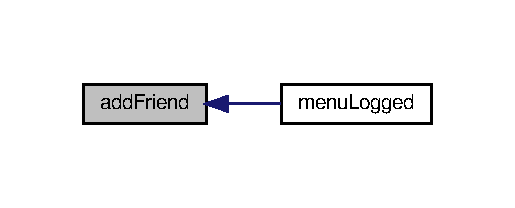
\includegraphics[width=247pt]{application_8h_a92aba65fab778922f928e9d9bf6475d6_icgraph}
\end{center}
\end{figure}
\mbox{\Hypertarget{application_8h_a58f4936001855f43fb36be2c1dda8542}\label{application_8h_a58f4936001855f43fb36be2c1dda8542}} 
\index{application.\+h@{application.\+h}!add\+Grade@{add\+Grade}}
\index{add\+Grade@{add\+Grade}!application.\+h@{application.\+h}}
\subsubsection{\texorpdfstring{add\+Grade()}{addGrade()}}
{\footnotesize\ttfamily unsigned add\+Grade (\begin{DoxyParamCaption}{ }\end{DoxyParamCaption})}

This function is asking the user to input a grade between 1-\/5 and has a validation. \begin{DoxyReturn}{Returns}
unsigned(grade) 
\end{DoxyReturn}
Here is the caller graph for this function\+:\nopagebreak
\begin{figure}[H]
\begin{center}
\leavevmode
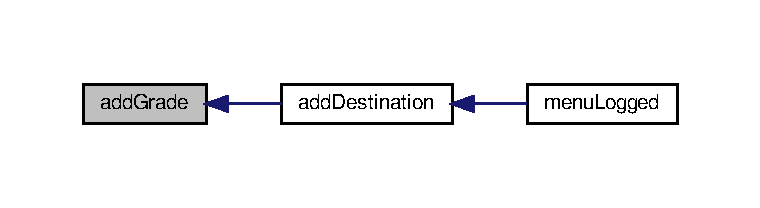
\includegraphics[width=350pt]{application_8h_a58f4936001855f43fb36be2c1dda8542_icgraph}
\end{center}
\end{figure}
\mbox{\Hypertarget{application_8h_a265d79751fc2100c17b58f15df75fed8}\label{application_8h_a265d79751fc2100c17b58f15df75fed8}} 
\index{application.\+h@{application.\+h}!add\+Location@{add\+Location}}
\index{add\+Location@{add\+Location}!application.\+h@{application.\+h}}
\subsubsection{\texorpdfstring{add\+Location()}{addLocation()}}
{\footnotesize\ttfamily string add\+Location (\begin{DoxyParamCaption}{ }\end{DoxyParamCaption})}

This function is asking the user for the location of the trip. \begin{DoxyReturn}{Returns}
string(location) 
\end{DoxyReturn}
Here is the caller graph for this function\+:\nopagebreak
\begin{figure}[H]
\begin{center}
\leavevmode
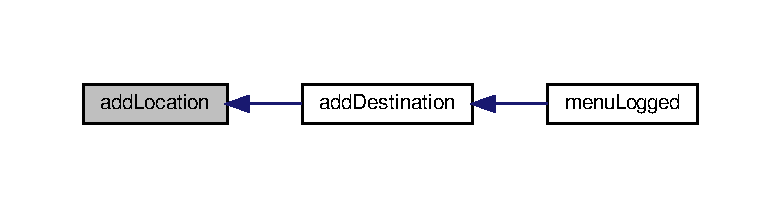
\includegraphics[width=350pt]{application_8h_a265d79751fc2100c17b58f15df75fed8_icgraph}
\end{center}
\end{figure}
\mbox{\Hypertarget{application_8h_a3fd32a66da2ec32c0823ad407e7d1f62}\label{application_8h_a3fd32a66da2ec32c0823ad407e7d1f62}} 
\index{application.\+h@{application.\+h}!add\+Photos@{add\+Photos}}
\index{add\+Photos@{add\+Photos}!application.\+h@{application.\+h}}
\subsubsection{\texorpdfstring{add\+Photos()}{addPhotos()}}
{\footnotesize\ttfamily vector$<$ string $>$ add\+Photos (\begin{DoxyParamCaption}\item[{int}]{num\+Photos }\end{DoxyParamCaption})}

This function is asking the user to input the name of the photos that he\textquotesingle{}d like to add to the database. Beforewards the user has to choose what the extenstions of the photos are going to be. \begin{DoxyReturn}{Returns}
vector$<$string$>$(photos) 
\end{DoxyReturn}

\begin{DoxyParams}{Parameters}
{\em int} & num\+Photos \\
\hline
\end{DoxyParams}
Here is the caller graph for this function\+:\nopagebreak
\begin{figure}[H]
\begin{center}
\leavevmode
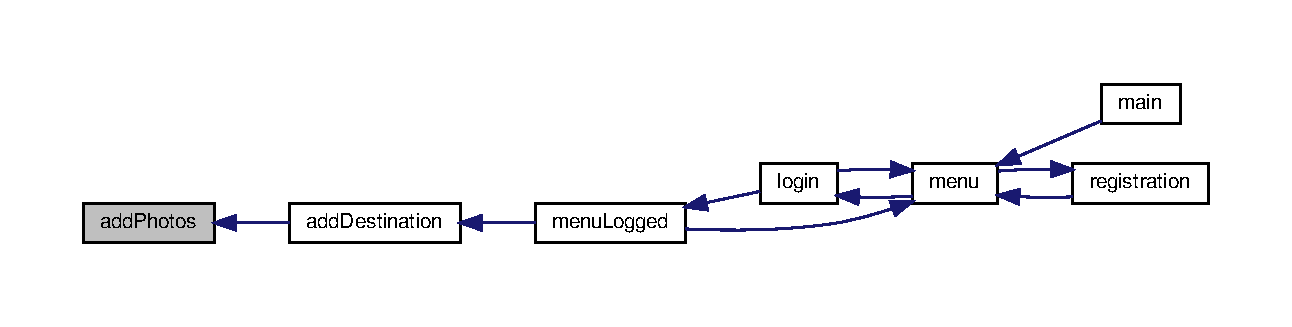
\includegraphics[width=350pt]{application_8h_a3fd32a66da2ec32c0823ad407e7d1f62_icgraph}
\end{center}
\end{figure}
\mbox{\Hypertarget{application_8h_a9066e8999df2f39d7ffeb81176fb14d4}\label{application_8h_a9066e8999df2f39d7ffeb81176fb14d4}} 
\index{application.\+h@{application.\+h}!add\+Start\+Date@{add\+Start\+Date}}
\index{add\+Start\+Date@{add\+Start\+Date}!application.\+h@{application.\+h}}
\subsubsection{\texorpdfstring{add\+Start\+Date()}{addStartDate()}}
{\footnotesize\ttfamily \hyperlink{class_date}{Date} add\+Start\+Date (\begin{DoxyParamCaption}{ }\end{DoxyParamCaption})}

This function is asking the user to input the start date and is initializing an object of type \hyperlink{class_date}{Date}. \begin{DoxyReturn}{Returns}
\hyperlink{class_date}{Date(start date)} 
\end{DoxyReturn}
Here is the caller graph for this function\+:\nopagebreak
\begin{figure}[H]
\begin{center}
\leavevmode
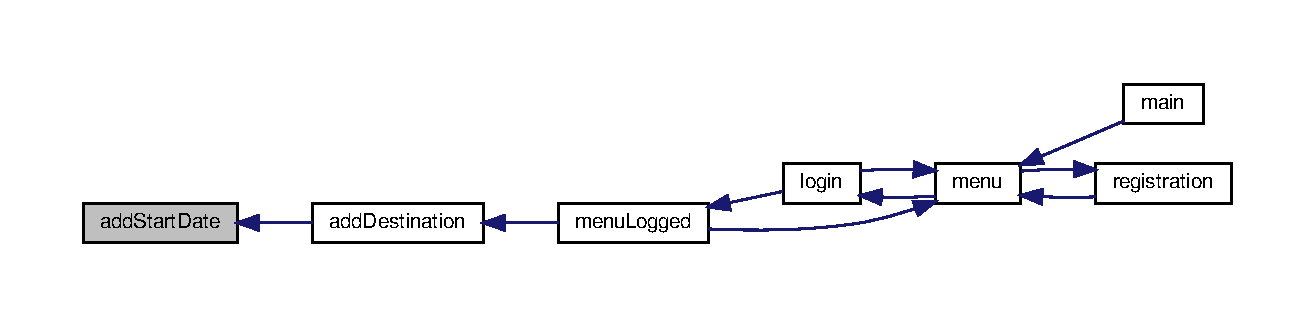
\includegraphics[width=350pt]{application_8h_a9066e8999df2f39d7ffeb81176fb14d4_icgraph}
\end{center}
\end{figure}
\mbox{\Hypertarget{application_8h_a3ca98c5244a06fb6199d64f44b6a2fa4}\label{application_8h_a3ca98c5244a06fb6199d64f44b6a2fa4}} 
\index{application.\+h@{application.\+h}!destination\+To\+File@{destination\+To\+File}}
\index{destination\+To\+File@{destination\+To\+File}!application.\+h@{application.\+h}}
\subsubsection{\texorpdfstring{destination\+To\+File()}{destinationToFile()}}
{\footnotesize\ttfamily void destination\+To\+File (\begin{DoxyParamCaption}\item[{const \hyperlink{class_user}{User} \&}]{logged\+In\+User,  }\item[{const \hyperlink{class_destination}{Destination} \&}]{being\+Added,  }\item[{int}]{num\+Photos }\end{DoxyParamCaption})}

The function accepts two object one ot type \hyperlink{class_destination}{Destination} and one of type \hyperlink{class_user}{User}. Afterwards is using the getters of class Destinaiton to save the destination to the accepted \hyperlink{class_user}{User}\textquotesingle{}s databse and to a file called \char`\"{}destinations.\+csv\char`\"{} which is used to get information about a destination. 
\begin{DoxyParams}{Parameters}
{\em const} & \hyperlink{class_user}{User}\& loged\+In\+User \\
\hline
{\em const} & \hyperlink{class_destination}{Destination}\& being\+Added \\
\hline
\end{DoxyParams}
Here is the call graph for this function\+:\nopagebreak
\begin{figure}[H]
\begin{center}
\leavevmode
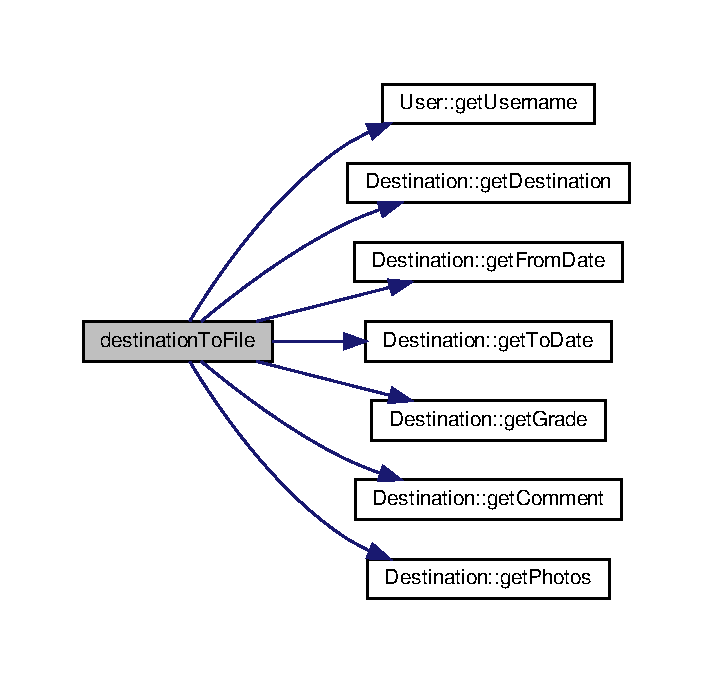
\includegraphics[width=342pt]{application_8h_a3ca98c5244a06fb6199d64f44b6a2fa4_cgraph}
\end{center}
\end{figure}
Here is the caller graph for this function\+:\nopagebreak
\begin{figure}[H]
\begin{center}
\leavevmode
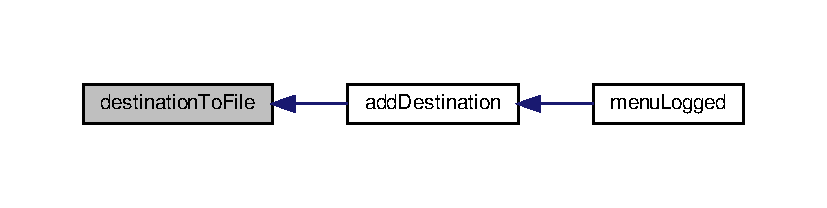
\includegraphics[width=350pt]{application_8h_a3ca98c5244a06fb6199d64f44b6a2fa4_icgraph}
\end{center}
\end{figure}
\mbox{\Hypertarget{application_8h_adf656ece2632a1013b0e510fbb0ac529}\label{application_8h_adf656ece2632a1013b0e510fbb0ac529}} 
\index{application.\+h@{application.\+h}!user\+To\+File@{user\+To\+File}}
\index{user\+To\+File@{user\+To\+File}!application.\+h@{application.\+h}}
\subsubsection{\texorpdfstring{user\+To\+File()}{userToFile()}}
{\footnotesize\ttfamily void user\+To\+File (\begin{DoxyParamCaption}\item[{const \hyperlink{class_user}{User} \&}]{being\+Reg }\end{DoxyParamCaption})}

The function accepts \hyperlink{class_user}{User} and though the getter\textquotesingle{}s method is saving the user\textquotesingle{}s username, password and email to users.\+db file and creates his own database file. 
\begin{DoxyParams}{Parameters}
{\em const} & \hyperlink{class_user}{User}\& being\+Reg \\
\hline
\end{DoxyParams}
Here is the call graph for this function\+:\nopagebreak
\begin{figure}[H]
\begin{center}
\leavevmode
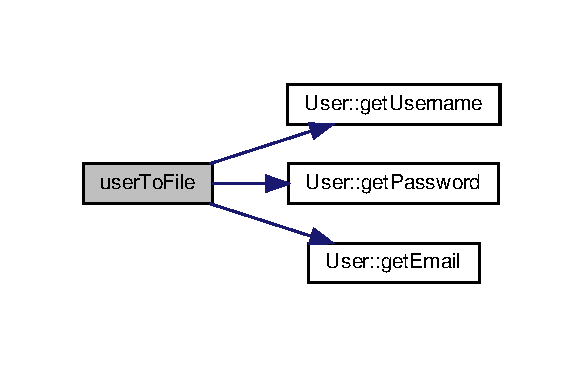
\includegraphics[width=280pt]{application_8h_adf656ece2632a1013b0e510fbb0ac529_cgraph}
\end{center}
\end{figure}
Here is the caller graph for this function\+:\nopagebreak
\begin{figure}[H]
\begin{center}
\leavevmode
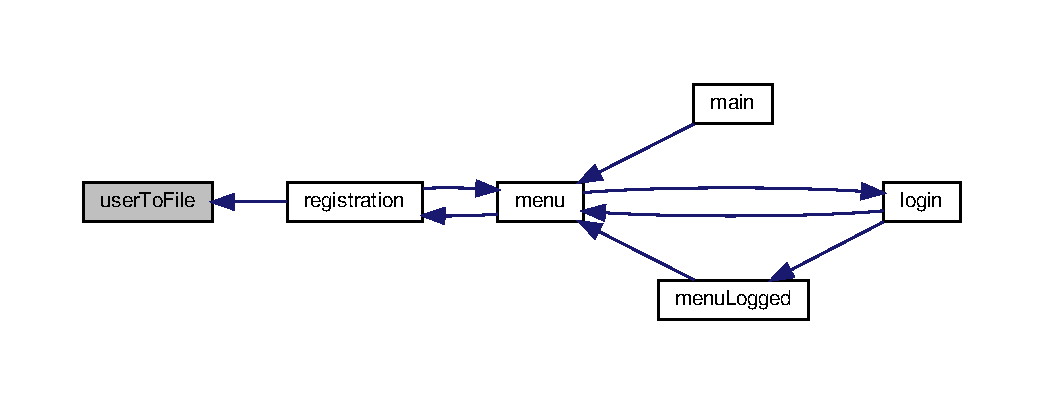
\includegraphics[width=350pt]{application_8h_adf656ece2632a1013b0e510fbb0ac529_icgraph}
\end{center}
\end{figure}

\hypertarget{date_8cpp}{}\section{date.\+cpp File Reference}
\label{date_8cpp}\index{date.\+cpp@{date.\+cpp}}
{\ttfamily \#include \char`\"{}date.\+h\char`\"{}}\newline
Include dependency graph for date.\+cpp\+:\nopagebreak
\begin{figure}[H]
\begin{center}
\leavevmode
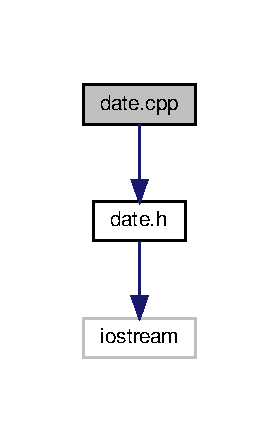
\includegraphics[width=134pt]{date_8cpp__incl}
\end{center}
\end{figure}
\subsection*{Functions}
\begin{DoxyCompactItemize}
\item 
ostream \& \hyperlink{date_8cpp_affced1a8a8f9f0e9dd009af0a22dfe33}{operator$<$$<$} (ostream \&fout, const \hyperlink{class_date}{Date} \&dt)
\end{DoxyCompactItemize}


\subsection{Function Documentation}
\mbox{\Hypertarget{date_8cpp_affced1a8a8f9f0e9dd009af0a22dfe33}\label{date_8cpp_affced1a8a8f9f0e9dd009af0a22dfe33}} 
\index{date.\+cpp@{date.\+cpp}!operator$<$$<$@{operator$<$$<$}}
\index{operator$<$$<$@{operator$<$$<$}!date.\+cpp@{date.\+cpp}}
\subsubsection{\texorpdfstring{operator$<$$<$()}{operator<<()}}
{\footnotesize\ttfamily ostream\& operator$<$$<$ (\begin{DoxyParamCaption}\item[{ostream \&}]{fout,  }\item[{const \hyperlink{class_date}{Date} \&}]{dt }\end{DoxyParamCaption})}

Overloaded operator$<$$<$. Here is the call graph for this function\+:\nopagebreak
\begin{figure}[H]
\begin{center}
\leavevmode
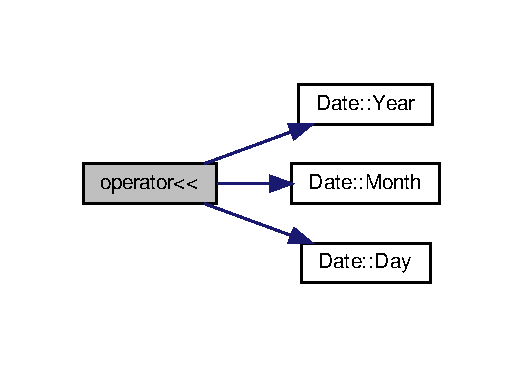
\includegraphics[width=251pt]{date_8cpp_affced1a8a8f9f0e9dd009af0a22dfe33_cgraph}
\end{center}
\end{figure}
Here is the caller graph for this function\+:\nopagebreak
\begin{figure}[H]
\begin{center}
\leavevmode
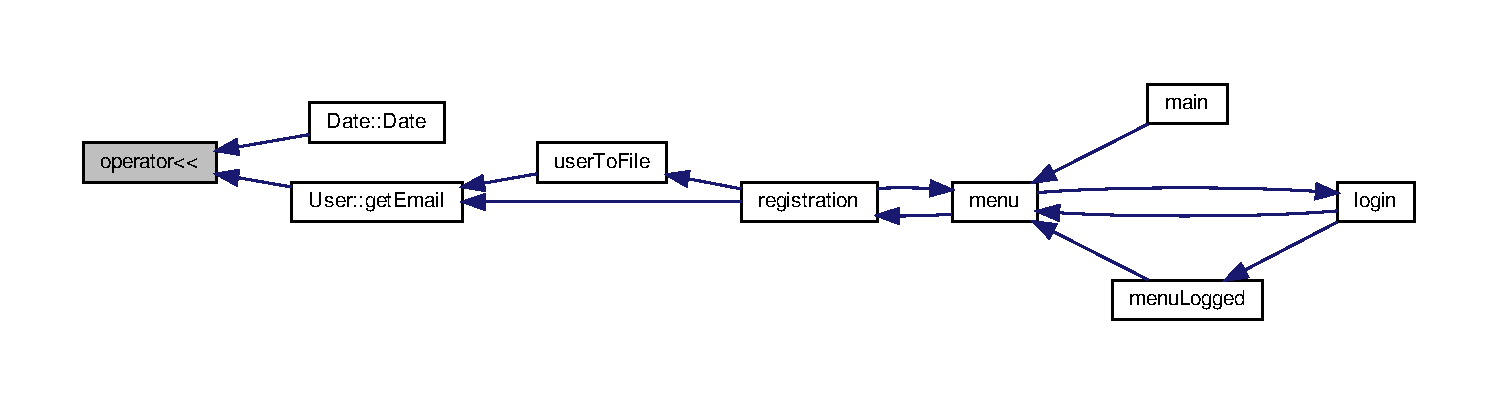
\includegraphics[width=350pt]{date_8cpp_affced1a8a8f9f0e9dd009af0a22dfe33_icgraph}
\end{center}
\end{figure}

\hypertarget{date_8h}{}\section{date.\+h File Reference}
\label{date_8h}\index{date.\+h@{date.\+h}}
{\ttfamily \#include $<$iostream$>$}\newline
Include dependency graph for date.\+h\+:\nopagebreak
\begin{figure}[H]
\begin{center}
\leavevmode
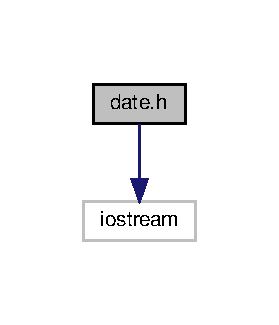
\includegraphics[width=134pt]{date_8h__incl}
\end{center}
\end{figure}
This graph shows which files directly or indirectly include this file\+:\nopagebreak
\begin{figure}[H]
\begin{center}
\leavevmode
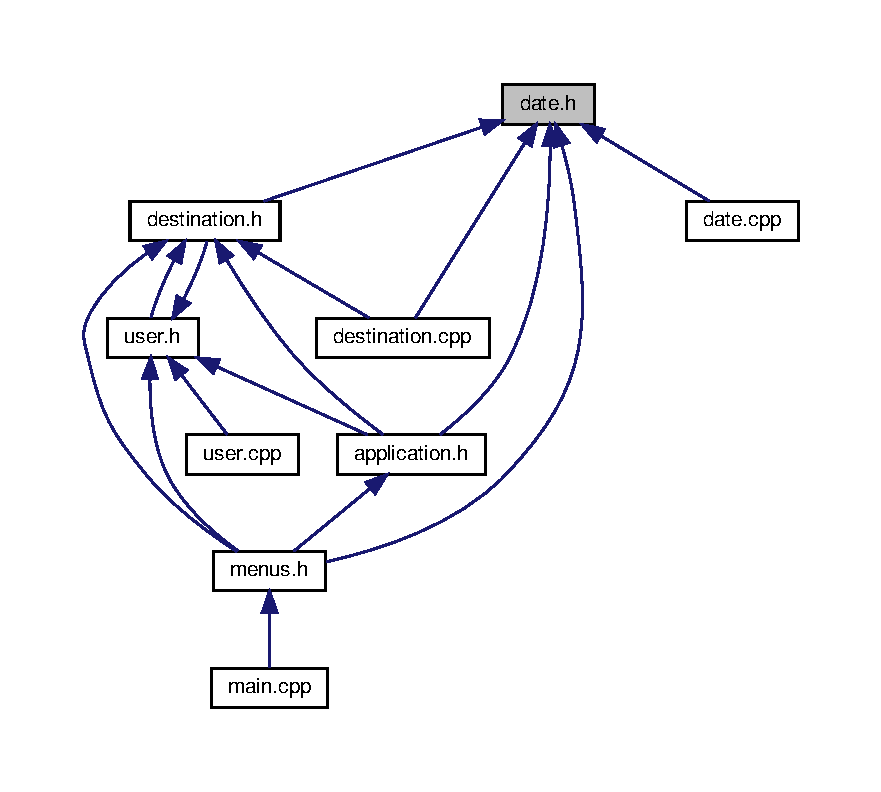
\includegraphics[width=350pt]{date_8h__dep__incl}
\end{center}
\end{figure}
\subsection*{Classes}
\begin{DoxyCompactItemize}
\item 
class \hyperlink{class_date}{Date}
\begin{DoxyCompactList}\small\item\em A date class. \end{DoxyCompactList}\end{DoxyCompactItemize}

\hypertarget{destination_8cpp}{}\section{destination.\+cpp File Reference}
\label{destination_8cpp}\index{destination.\+cpp@{destination.\+cpp}}
{\ttfamily \#include \char`\"{}destination.\+h\char`\"{}}\newline
{\ttfamily \#include \char`\"{}date.\+h\char`\"{}}\newline
Include dependency graph for destination.\+cpp\+:\nopagebreak
\begin{figure}[H]
\begin{center}
\leavevmode
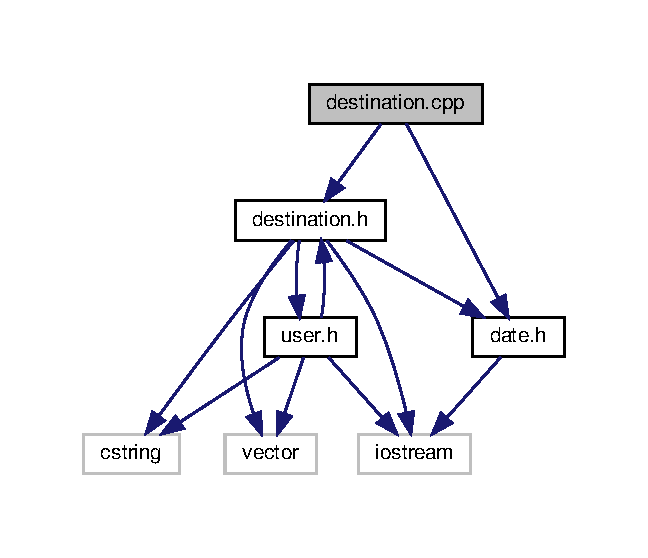
\includegraphics[width=311pt]{destination_8cpp__incl}
\end{center}
\end{figure}

\hypertarget{destination_8h}{}\section{destination.\+h File Reference}
\label{destination_8h}\index{destination.\+h@{destination.\+h}}
{\ttfamily \#include $<$iostream$>$}\newline
{\ttfamily \#include $<$cstring$>$}\newline
{\ttfamily \#include $<$vector$>$}\newline
{\ttfamily \#include \char`\"{}user.\+h\char`\"{}}\newline
{\ttfamily \#include \char`\"{}date.\+h\char`\"{}}\newline
Include dependency graph for destination.\+h\+:\nopagebreak
\begin{figure}[H]
\begin{center}
\leavevmode
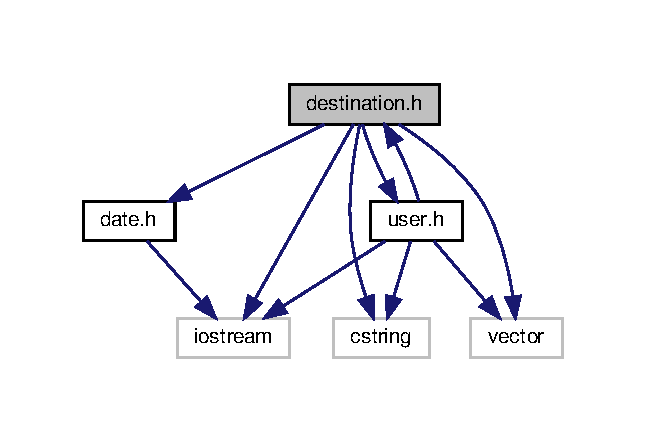
\includegraphics[width=310pt]{destination_8h__incl}
\end{center}
\end{figure}
This graph shows which files directly or indirectly include this file\+:\nopagebreak
\begin{figure}[H]
\begin{center}
\leavevmode
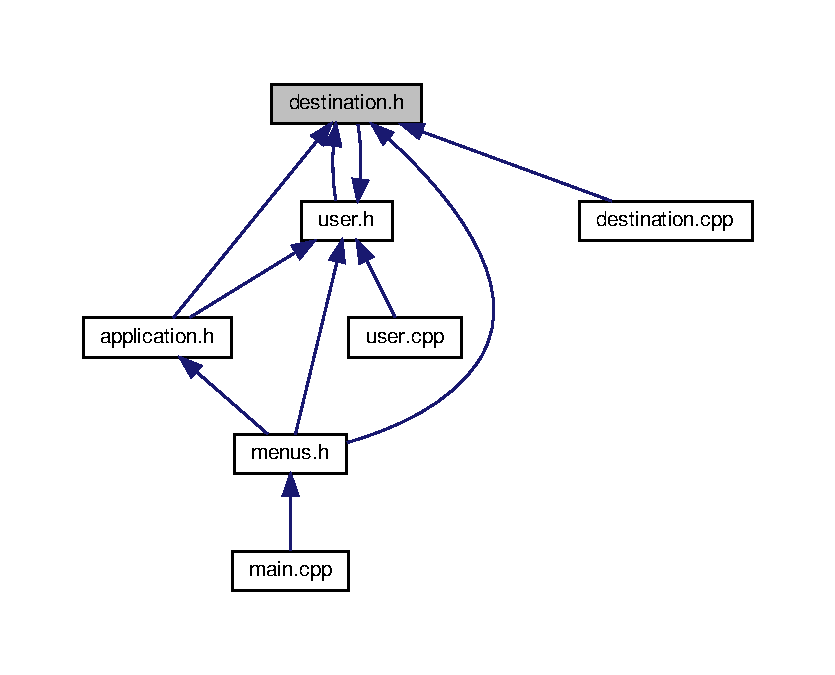
\includegraphics[width=350pt]{destination_8h__dep__incl}
\end{center}
\end{figure}
\subsection*{Classes}
\begin{DoxyCompactItemize}
\item 
class \hyperlink{class_destination}{Destination}
\begin{DoxyCompactList}\small\item\em A destination class. \end{DoxyCompactList}\end{DoxyCompactItemize}

\hypertarget{main_8cpp}{}\section{main.\+cpp File Reference}
\label{main_8cpp}\index{main.\+cpp@{main.\+cpp}}
{\ttfamily \#include $<$iostream$>$}\newline
{\ttfamily \#include \char`\"{}menus.\+h\char`\"{}}\newline
Include dependency graph for main.\+cpp\+:\nopagebreak
\begin{figure}[H]
\begin{center}
\leavevmode
\includegraphics[width=350pt]{main_8cpp__incl}
\end{center}
\end{figure}
\subsection*{Functions}
\begin{DoxyCompactItemize}
\item 
int \hyperlink{main_8cpp_ae66f6b31b5ad750f1fe042a706a4e3d4}{main} ()
\end{DoxyCompactItemize}


\subsection{Function Documentation}
\mbox{\Hypertarget{main_8cpp_ae66f6b31b5ad750f1fe042a706a4e3d4}\label{main_8cpp_ae66f6b31b5ad750f1fe042a706a4e3d4}} 
\index{main.\+cpp@{main.\+cpp}!main@{main}}
\index{main@{main}!main.\+cpp@{main.\+cpp}}
\subsubsection{\texorpdfstring{main()}{main()}}
{\footnotesize\ttfamily int main (\begin{DoxyParamCaption}{ }\end{DoxyParamCaption})}

Here is the call graph for this function\+:\nopagebreak
\begin{figure}[H]
\begin{center}
\leavevmode
\includegraphics[width=350pt]{main_8cpp_ae66f6b31b5ad750f1fe042a706a4e3d4_cgraph}
\end{center}
\end{figure}

\hypertarget{menus_8h}{}\section{menus.\+h File Reference}
\label{menus_8h}\index{menus.\+h@{menus.\+h}}
{\ttfamily \#include $<$iostream$>$}\newline
{\ttfamily \#include $<$fstream$>$}\newline
{\ttfamily \#include $<$string$>$}\newline
{\ttfamily \#include $<$cstdlib$>$}\newline
{\ttfamily \#include \char`\"{}user.\+h\char`\"{}}\newline
{\ttfamily \#include \char`\"{}destination.\+h\char`\"{}}\newline
{\ttfamily \#include \char`\"{}date.\+h\char`\"{}}\newline
{\ttfamily \#include \char`\"{}read\+File.\+h\char`\"{}}\newline
{\ttfamily \#include \char`\"{}application.\+h\char`\"{}}\newline
Include dependency graph for menus.\+h\+:\nopagebreak
\begin{figure}[H]
\begin{center}
\leavevmode
\includegraphics[width=350pt]{menus_8h__incl}
\end{center}
\end{figure}
This graph shows which files directly or indirectly include this file\+:\nopagebreak
\begin{figure}[H]
\begin{center}
\leavevmode
\includegraphics[width=136pt]{menus_8h__dep__incl}
\end{center}
\end{figure}
\subsection*{Functions}
\begin{DoxyCompactItemize}
\item 
void \hyperlink{menus_8h_a714c83c6898e18f73621626df5bb59c3}{registration} ()
\item 
void \hyperlink{menus_8h_af76b7b46958dabf5e4ee9a492f0ec3fa}{login} ()
\item 
void \hyperlink{menus_8h_a2a0e843767aeea4f433a28b9c54f573a}{menu} ()
\item 
void \hyperlink{menus_8h_a1f5d479249cf7405f3ef126b1e042d2b}{menu\+Logged} (const \hyperlink{class_user}{User} \&logged\+In\+User)
\end{DoxyCompactItemize}


\subsection{Function Documentation}
\mbox{\Hypertarget{menus_8h_af76b7b46958dabf5e4ee9a492f0ec3fa}\label{menus_8h_af76b7b46958dabf5e4ee9a492f0ec3fa}} 
\index{menus.\+h@{menus.\+h}!login@{login}}
\index{login@{login}!menus.\+h@{menus.\+h}}
\subsubsection{\texorpdfstring{login()}{login()}}
{\footnotesize\ttfamily void login (\begin{DoxyParamCaption}{ }\end{DoxyParamCaption})}

This function is used when you try to log in. The user inserts two strings(username and password). Firstly, the username is checked whether such a user exists and if it exists, then the function checkes whether the inserted password matches the inserted username. Here is the call graph for this function\+:\nopagebreak
\begin{figure}[H]
\begin{center}
\leavevmode
\includegraphics[width=350pt]{menus_8h_af76b7b46958dabf5e4ee9a492f0ec3fa_cgraph}
\end{center}
\end{figure}
Here is the caller graph for this function\+:\nopagebreak
\begin{figure}[H]
\begin{center}
\leavevmode
\includegraphics[width=302pt]{menus_8h_af76b7b46958dabf5e4ee9a492f0ec3fa_icgraph}
\end{center}
\end{figure}
\mbox{\Hypertarget{menus_8h_a2a0e843767aeea4f433a28b9c54f573a}\label{menus_8h_a2a0e843767aeea4f433a28b9c54f573a}} 
\index{menus.\+h@{menus.\+h}!menu@{menu}}
\index{menu@{menu}!menus.\+h@{menus.\+h}}
\subsubsection{\texorpdfstring{menu()}{menu()}}
{\footnotesize\ttfamily void menu (\begin{DoxyParamCaption}{ }\end{DoxyParamCaption})}

The functions prints R\+E\+G\+I\+S\+T\+ER, L\+O\+G\+IN OR E\+X\+IT and awaits value to be inputted in order to know action to execute. Here is the call graph for this function\+:\nopagebreak
\begin{figure}[H]
\begin{center}
\leavevmode
\includegraphics[width=350pt]{menus_8h_a2a0e843767aeea4f433a28b9c54f573a_cgraph}
\end{center}
\end{figure}
Here is the caller graph for this function\+:\nopagebreak
\begin{figure}[H]
\begin{center}
\leavevmode
\includegraphics[width=302pt]{menus_8h_a2a0e843767aeea4f433a28b9c54f573a_icgraph}
\end{center}
\end{figure}
\mbox{\Hypertarget{menus_8h_a1f5d479249cf7405f3ef126b1e042d2b}\label{menus_8h_a1f5d479249cf7405f3ef126b1e042d2b}} 
\index{menus.\+h@{menus.\+h}!menu\+Logged@{menu\+Logged}}
\index{menu\+Logged@{menu\+Logged}!menus.\+h@{menus.\+h}}
\subsubsection{\texorpdfstring{menu\+Logged()}{menuLogged()}}
{\footnotesize\ttfamily void menu\+Logged (\begin{DoxyParamCaption}\item[{const \hyperlink{class_user}{User} \&}]{logged\+In\+User }\end{DoxyParamCaption})}

The function is called when the process of logging in is successful. It prints all possible functionalities of the program(adding a trip, adding a friend, displaying infromation and etc...). It also awaits input in order to know which finction to call. 
\begin{DoxyParams}{Parameters}
{\em const} & \hyperlink{class_user}{User}\& logged\+In\+User \\
\hline
\end{DoxyParams}
Here is the call graph for this function\+:\nopagebreak
\begin{figure}[H]
\begin{center}
\leavevmode
\includegraphics[width=350pt]{menus_8h_a1f5d479249cf7405f3ef126b1e042d2b_cgraph}
\end{center}
\end{figure}
Here is the caller graph for this function\+:\nopagebreak
\begin{figure}[H]
\begin{center}
\leavevmode
\includegraphics[width=350pt]{menus_8h_a1f5d479249cf7405f3ef126b1e042d2b_icgraph}
\end{center}
\end{figure}
\mbox{\Hypertarget{menus_8h_a714c83c6898e18f73621626df5bb59c3}\label{menus_8h_a714c83c6898e18f73621626df5bb59c3}} 
\index{menus.\+h@{menus.\+h}!registration@{registration}}
\index{registration@{registration}!menus.\+h@{menus.\+h}}
\subsubsection{\texorpdfstring{registration()}{registration()}}
{\footnotesize\ttfamily void registration (\begin{DoxyParamCaption}{ }\end{DoxyParamCaption})}

This function is used to create a profile. Firstly, an object of type \hyperlink{class_user}{User} is created with default values(empty strings for username, password and email). Then asking the user to input these values and through the setters of class \hyperlink{class_user}{User} the inserted values are assigned to the object. There is a validation to prevent registering two profiles with the same username or email. Moreover two files are being opened and through the getters of class \hyperlink{class_user}{User} all the data of the object is saved into the files. Here is the call graph for this function\+:\nopagebreak
\begin{figure}[H]
\begin{center}
\leavevmode
\includegraphics[width=350pt]{menus_8h_a714c83c6898e18f73621626df5bb59c3_cgraph}
\end{center}
\end{figure}
Here is the caller graph for this function\+:\nopagebreak
\begin{figure}[H]
\begin{center}
\leavevmode
\includegraphics[width=350pt]{menus_8h_a714c83c6898e18f73621626df5bb59c3_icgraph}
\end{center}
\end{figure}

\hypertarget{read_file_8h}{}\section{read\+File.\+h File Reference}
\label{read_file_8h}\index{read\+File.\+h@{read\+File.\+h}}
{\ttfamily \#include $<$iostream$>$}\newline
{\ttfamily \#include $<$iomanip$>$}\newline
{\ttfamily \#include $<$fstream$>$}\newline
{\ttfamily \#include $<$sstream$>$}\newline
{\ttfamily \#include $<$vector$>$}\newline
Include dependency graph for read\+File.\+h\+:\nopagebreak
\begin{figure}[H]
\begin{center}
\leavevmode
\includegraphics[width=350pt]{read_file_8h__incl}
\end{center}
\end{figure}
This graph shows which files directly or indirectly include this file\+:\nopagebreak
\begin{figure}[H]
\begin{center}
\leavevmode
\includegraphics[width=151pt]{read_file_8h__dep__incl}
\end{center}
\end{figure}
\subsection*{Typedefs}
\begin{DoxyCompactItemize}
\item 
\mbox{\Hypertarget{read_file_8h_ac4ba865c2f8f6f90e3c64552279f3d21}\label{read_file_8h_ac4ba865c2f8f6f90e3c64552279f3d21}} 
using {\bfseries vec} = vector$<$ string $>$
\item 
\mbox{\Hypertarget{read_file_8h_a869e2a5deeb3daa4c82d6bc91cf20d92}\label{read_file_8h_a869e2a5deeb3daa4c82d6bc91cf20d92}} 
using {\bfseries matrix} = vector$<$ vec $>$
\end{DoxyCompactItemize}
\subsection*{Functions}
\begin{DoxyCompactItemize}
\item 
matrix \hyperlink{read_file_8h_a4d05aa34d631728e8dabfe1d9ddbdd69}{file\+To\+Matrix} (const string \&filename)
\item 
void \hyperlink{read_file_8h_ae04ba1e32f1dfd605e53f54c39b365fd}{display\+Matrix} (const matrix \&mat)
\item 
\mbox{\Hypertarget{read_file_8h_a71844c343db9878de02bcddae45947dd}\label{read_file_8h_a71844c343db9878de02bcddae45947dd}} 
bool {\bfseries username\+Matches\+Password} (const matrix \&mat, const string \&username, const string \&password)
\item 
void \hyperlink{read_file_8h_a3c27433c2ddbe1b8010a05a86cd21734}{average\+Grade\+Destination} (const matrix \&mat, const string \&destination)
\item 
bool \hyperlink{read_file_8h_ab6bce9fa2a7660f6f3ddcef5a4f7b906}{is\+Existing} (const matrix \&mat, const string \&check, int col)
\item 
int \hyperlink{read_file_8h_a331b6af63862d2ae3ad6abf71b0de381}{row\+Of\+Username} (const matrix \&mat, const string \&username)
\item 
int \hyperlink{read_file_8h_a4fc77629ec6e6556b5dc4dd8efa6f36c}{number\+Of\+Rows\+In\+File} (const matrix \&mat)
\item 
void \hyperlink{read_file_8h_ac9d4f6924d2d252073454cbe2dfd9895}{display\+Friends} (const matrix \&mat, const string \&username)
\item 
bool \hyperlink{read_file_8h_a6b426552d2ff56784a167e799da87688}{is\+Already\+Friend} (const matrix \&mat, const string \&friend\+To\+Be\+Added, const string \&username)
\item 
void \hyperlink{read_file_8h_af9f2aec2ef105eff0f596a9b91ae98b3}{display\+Friends\+Destionations} (const string \&logged\+In\+Username)
\item 
void \hyperlink{read_file_8h_a3c8596d363a098e38a811efab756aa5b}{display\+Info\+For\+Particular\+Destination} ()
\end{DoxyCompactItemize}


\subsection{Function Documentation}
\mbox{\Hypertarget{read_file_8h_a3c27433c2ddbe1b8010a05a86cd21734}\label{read_file_8h_a3c27433c2ddbe1b8010a05a86cd21734}} 
\index{read\+File.\+h@{read\+File.\+h}!average\+Grade\+Destination@{average\+Grade\+Destination}}
\index{average\+Grade\+Destination@{average\+Grade\+Destination}!read\+File.\+h@{read\+File.\+h}}
\subsubsection{\texorpdfstring{average\+Grade\+Destination()}{averageGradeDestination()}}
{\footnotesize\ttfamily void average\+Grade\+Destination (\begin{DoxyParamCaption}\item[{const matrix \&}]{mat,  }\item[{const string \&}]{destination }\end{DoxyParamCaption})}

This function is accepting a string(destination/location) and checking in the database how many times the the location has been visited and returns the average grade from all users. 
\begin{DoxyParams}{Parameters}
{\em const} & matrix\& mat \\
\hline
{\em const} & string\& destination \\
\hline
\end{DoxyParams}
Here is the caller graph for this function\+:\nopagebreak
\begin{figure}[H]
\begin{center}
\leavevmode
\includegraphics[width=315pt]{read_file_8h_a3c27433c2ddbe1b8010a05a86cd21734_icgraph}
\end{center}
\end{figure}
\mbox{\Hypertarget{read_file_8h_ac9d4f6924d2d252073454cbe2dfd9895}\label{read_file_8h_ac9d4f6924d2d252073454cbe2dfd9895}} 
\index{read\+File.\+h@{read\+File.\+h}!display\+Friends@{display\+Friends}}
\index{display\+Friends@{display\+Friends}!read\+File.\+h@{read\+File.\+h}}
\subsubsection{\texorpdfstring{display\+Friends()}{displayFriends()}}
{\footnotesize\ttfamily void display\+Friends (\begin{DoxyParamCaption}\item[{const matrix \&}]{mat,  }\item[{const string \&}]{username }\end{DoxyParamCaption})}

This function is accepting a string(username) and is displaying his friends. 
\begin{DoxyParams}{Parameters}
{\em const} & matrix\& mat \\
\hline
{\em const} & string\& username \\
\hline
\end{DoxyParams}
Here is the caller graph for this function\+:\nopagebreak
\begin{figure}[H]
\begin{center}
\leavevmode
\includegraphics[width=268pt]{read_file_8h_ac9d4f6924d2d252073454cbe2dfd9895_icgraph}
\end{center}
\end{figure}
\mbox{\Hypertarget{read_file_8h_af9f2aec2ef105eff0f596a9b91ae98b3}\label{read_file_8h_af9f2aec2ef105eff0f596a9b91ae98b3}} 
\index{read\+File.\+h@{read\+File.\+h}!display\+Friends\+Destionations@{display\+Friends\+Destionations}}
\index{display\+Friends\+Destionations@{display\+Friends\+Destionations}!read\+File.\+h@{read\+File.\+h}}
\subsubsection{\texorpdfstring{display\+Friends\+Destionations()}{displayFriendsDestionations()}}
{\footnotesize\ttfamily void display\+Friends\+Destionations (\begin{DoxyParamCaption}\item[{const string \&}]{logged\+In\+Username }\end{DoxyParamCaption})}

Displays all places where the friends of the loggedin user have been alonside with their comments about the trip. 
\begin{DoxyParams}{Parameters}
{\em const} & string\& logged\+In\+Username \\
\hline
\end{DoxyParams}
Here is the call graph for this function\+:\nopagebreak
\begin{figure}[H]
\begin{center}
\leavevmode
\includegraphics[width=324pt]{read_file_8h_af9f2aec2ef105eff0f596a9b91ae98b3_cgraph}
\end{center}
\end{figure}
Here is the caller graph for this function\+:\nopagebreak
\begin{figure}[H]
\begin{center}
\leavevmode
\includegraphics[width=328pt]{read_file_8h_af9f2aec2ef105eff0f596a9b91ae98b3_icgraph}
\end{center}
\end{figure}
\mbox{\Hypertarget{read_file_8h_a3c8596d363a098e38a811efab756aa5b}\label{read_file_8h_a3c8596d363a098e38a811efab756aa5b}} 
\index{read\+File.\+h@{read\+File.\+h}!display\+Info\+For\+Particular\+Destination@{display\+Info\+For\+Particular\+Destination}}
\index{display\+Info\+For\+Particular\+Destination@{display\+Info\+For\+Particular\+Destination}!read\+File.\+h@{read\+File.\+h}}
\subsubsection{\texorpdfstring{display\+Info\+For\+Particular\+Destination()}{displayInfoForParticularDestination()}}
{\footnotesize\ttfamily void display\+Info\+For\+Particular\+Destination (\begin{DoxyParamCaption}{ }\end{DoxyParamCaption})}

The function is accepting a string(location) and displays all users who have been to this location and their grade. Here is the call graph for this function\+:\nopagebreak
\begin{figure}[H]
\begin{center}
\leavevmode
\includegraphics[width=303pt]{read_file_8h_a3c8596d363a098e38a811efab756aa5b_cgraph}
\end{center}
\end{figure}
Here is the caller graph for this function\+:\nopagebreak
\begin{figure}[H]
\begin{center}
\leavevmode
\includegraphics[width=307pt]{read_file_8h_a3c8596d363a098e38a811efab756aa5b_icgraph}
\end{center}
\end{figure}
\mbox{\Hypertarget{read_file_8h_ae04ba1e32f1dfd605e53f54c39b365fd}\label{read_file_8h_ae04ba1e32f1dfd605e53f54c39b365fd}} 
\index{read\+File.\+h@{read\+File.\+h}!display\+Matrix@{display\+Matrix}}
\index{display\+Matrix@{display\+Matrix}!read\+File.\+h@{read\+File.\+h}}
\subsubsection{\texorpdfstring{display\+Matrix()}{displayMatrix()}}
{\footnotesize\ttfamily void display\+Matrix (\begin{DoxyParamCaption}\item[{const matrix \&}]{mat }\end{DoxyParamCaption})}

This function is displaying the table(matrix). 
\begin{DoxyParams}{Parameters}
{\em const} & matrix\& mat \\
\hline
\end{DoxyParams}
Here is the caller graph for this function\+:\nopagebreak
\begin{figure}[H]
\begin{center}
\leavevmode
\includegraphics[width=262pt]{read_file_8h_ae04ba1e32f1dfd605e53f54c39b365fd_icgraph}
\end{center}
\end{figure}
\mbox{\Hypertarget{read_file_8h_a4d05aa34d631728e8dabfe1d9ddbdd69}\label{read_file_8h_a4d05aa34d631728e8dabfe1d9ddbdd69}} 
\index{read\+File.\+h@{read\+File.\+h}!file\+To\+Matrix@{file\+To\+Matrix}}
\index{file\+To\+Matrix@{file\+To\+Matrix}!read\+File.\+h@{read\+File.\+h}}
\subsubsection{\texorpdfstring{file\+To\+Matrix()}{fileToMatrix()}}
{\footnotesize\ttfamily matrix file\+To\+Matrix (\begin{DoxyParamCaption}\item[{const string \&}]{filename }\end{DoxyParamCaption})}

The functions reads the information from the file named \char`\"{}filename\char`\"{} and is storing the information to a matrix(vector$<$vector$<$stirng$>$$>$). 
\begin{DoxyParams}{Parameters}
{\em filename} & \\
\hline
\end{DoxyParams}
\begin{DoxyReturn}{Returns}
matrix(vector$<$vector$<$string$>$$>$) with the information from the file \char`\"{}filename\char`\"{} 
\end{DoxyReturn}
Here is the caller graph for this function\+:\nopagebreak
\begin{figure}[H]
\begin{center}
\leavevmode
\includegraphics[width=350pt]{read_file_8h_a4d05aa34d631728e8dabfe1d9ddbdd69_icgraph}
\end{center}
\end{figure}
\mbox{\Hypertarget{read_file_8h_a6b426552d2ff56784a167e799da87688}\label{read_file_8h_a6b426552d2ff56784a167e799da87688}} 
\index{read\+File.\+h@{read\+File.\+h}!is\+Already\+Friend@{is\+Already\+Friend}}
\index{is\+Already\+Friend@{is\+Already\+Friend}!read\+File.\+h@{read\+File.\+h}}
\subsubsection{\texorpdfstring{is\+Already\+Friend()}{isAlreadyFriend()}}
{\footnotesize\ttfamily bool is\+Already\+Friend (\begin{DoxyParamCaption}\item[{const matrix \&}]{mat,  }\item[{const string \&}]{friend\+To\+Be\+Added,  }\item[{const string \&}]{username }\end{DoxyParamCaption})}

The function is checking whether the inserted string(friend\+To\+Be\+Added) is already in the friend list. 
\begin{DoxyParams}{Parameters}
{\em const} & matrix\& mat \\
\hline
{\em const} & string\& friend\+To\+Be\+Added \\
\hline
{\em const} & string\&username \\
\hline
\end{DoxyParams}
\begin{DoxyReturn}{Returns}
true or false 
\end{DoxyReturn}
Here is the caller graph for this function\+:\nopagebreak
\begin{figure}[H]
\begin{center}
\leavevmode
\includegraphics[width=350pt]{read_file_8h_a6b426552d2ff56784a167e799da87688_icgraph}
\end{center}
\end{figure}
\mbox{\Hypertarget{read_file_8h_ab6bce9fa2a7660f6f3ddcef5a4f7b906}\label{read_file_8h_ab6bce9fa2a7660f6f3ddcef5a4f7b906}} 
\index{read\+File.\+h@{read\+File.\+h}!is\+Existing@{is\+Existing}}
\index{is\+Existing@{is\+Existing}!read\+File.\+h@{read\+File.\+h}}
\subsubsection{\texorpdfstring{is\+Existing()}{isExisting()}}
{\footnotesize\ttfamily bool is\+Existing (\begin{DoxyParamCaption}\item[{const matrix \&}]{mat,  }\item[{const string \&}]{check,  }\item[{int}]{col }\end{DoxyParamCaption})}

This functions accepts a string and checks whether it is already in the database. The int col is used to check just a column from the matrix. This functions is used to prevent registering two profiles with the same username or email. 
\begin{DoxyParams}{Parameters}
{\em const} & matrix\& mat \\
\hline
{\em const} & string\& check \\
\hline
{\em int} & col \\
\hline
\end{DoxyParams}
\begin{DoxyReturn}{Returns}
true or false 
\end{DoxyReturn}
Here is the caller graph for this function\+:\nopagebreak
\begin{figure}[H]
\begin{center}
\leavevmode
\includegraphics[width=350pt]{read_file_8h_ab6bce9fa2a7660f6f3ddcef5a4f7b906_icgraph}
\end{center}
\end{figure}
\mbox{\Hypertarget{read_file_8h_a4fc77629ec6e6556b5dc4dd8efa6f36c}\label{read_file_8h_a4fc77629ec6e6556b5dc4dd8efa6f36c}} 
\index{read\+File.\+h@{read\+File.\+h}!number\+Of\+Rows\+In\+File@{number\+Of\+Rows\+In\+File}}
\index{number\+Of\+Rows\+In\+File@{number\+Of\+Rows\+In\+File}!read\+File.\+h@{read\+File.\+h}}
\subsubsection{\texorpdfstring{number\+Of\+Rows\+In\+File()}{numberOfRowsInFile()}}
{\footnotesize\ttfamily int number\+Of\+Rows\+In\+File (\begin{DoxyParamCaption}\item[{const matrix \&}]{mat }\end{DoxyParamCaption})}


\begin{DoxyParams}{Parameters}
{\em const} & matrix\& mat \\
\hline
\end{DoxyParams}
\begin{DoxyReturn}{Returns}
int(number of rows in the file) 
\end{DoxyReturn}
Here is the caller graph for this function\+:\nopagebreak
\begin{figure}[H]
\begin{center}
\leavevmode
\includegraphics[width=350pt]{read_file_8h_a4fc77629ec6e6556b5dc4dd8efa6f36c_icgraph}
\end{center}
\end{figure}
\mbox{\Hypertarget{read_file_8h_a331b6af63862d2ae3ad6abf71b0de381}\label{read_file_8h_a331b6af63862d2ae3ad6abf71b0de381}} 
\index{read\+File.\+h@{read\+File.\+h}!row\+Of\+Username@{row\+Of\+Username}}
\index{row\+Of\+Username@{row\+Of\+Username}!read\+File.\+h@{read\+File.\+h}}
\subsubsection{\texorpdfstring{row\+Of\+Username()}{rowOfUsername()}}
{\footnotesize\ttfamily int row\+Of\+Username (\begin{DoxyParamCaption}\item[{const matrix \&}]{mat,  }\item[{const string \&}]{username }\end{DoxyParamCaption})}

The function is accepting a string(username) and iterates through the file until the string is found and returns the number of the row. It is used when adding a friend in order to determine at which row should the new friend(username) be added. 
\begin{DoxyParams}{Parameters}
{\em const} & matrix\& mat \\
\hline
{\em const} & string\& username \\
\hline
\end{DoxyParams}
\begin{DoxyReturn}{Returns}
int(on which row in the file is the username) 
\end{DoxyReturn}
Here is the caller graph for this function\+:\nopagebreak
\begin{figure}[H]
\begin{center}
\leavevmode
\includegraphics[width=350pt]{read_file_8h_a331b6af63862d2ae3ad6abf71b0de381_icgraph}
\end{center}
\end{figure}

\hypertarget{user_8cpp}{}\section{user.\+cpp File Reference}
\label{user_8cpp}\index{user.\+cpp@{user.\+cpp}}
{\ttfamily \#include \char`\"{}user.\+h\char`\"{}}\newline
Include dependency graph for user.\+cpp\+:\nopagebreak
\begin{figure}[H]
\begin{center}
\leavevmode
\includegraphics[width=300pt]{user_8cpp__incl}
\end{center}
\end{figure}
\subsection*{Functions}
\begin{DoxyCompactItemize}
\item 
ostream \& \hyperlink{user_8cpp_acf1038a8d320684dc3fbdd5e4308e062}{operator$<$$<$} (ostream \&out, const \hyperlink{class_user}{User} \&user)
\item 
istream \& \hyperlink{user_8cpp_aae624f64cdd1af3b59c2443cffa82494}{operator$>$$>$} (istream \&in, \hyperlink{class_user}{User} \&user)
\end{DoxyCompactItemize}


\subsection{Function Documentation}
\mbox{\Hypertarget{user_8cpp_acf1038a8d320684dc3fbdd5e4308e062}\label{user_8cpp_acf1038a8d320684dc3fbdd5e4308e062}} 
\index{user.\+cpp@{user.\+cpp}!operator$<$$<$@{operator$<$$<$}}
\index{operator$<$$<$@{operator$<$$<$}!user.\+cpp@{user.\+cpp}}
\subsubsection{\texorpdfstring{operator$<$$<$()}{operator<<()}}
{\footnotesize\ttfamily ostream\& operator$<$$<$ (\begin{DoxyParamCaption}\item[{ostream \&}]{out,  }\item[{const \hyperlink{class_user}{User} \&}]{user }\end{DoxyParamCaption})}

Overloaded operator$<$$<$. \mbox{\Hypertarget{user_8cpp_aae624f64cdd1af3b59c2443cffa82494}\label{user_8cpp_aae624f64cdd1af3b59c2443cffa82494}} 
\index{user.\+cpp@{user.\+cpp}!operator$>$$>$@{operator$>$$>$}}
\index{operator$>$$>$@{operator$>$$>$}!user.\+cpp@{user.\+cpp}}
\subsubsection{\texorpdfstring{operator$>$$>$()}{operator>>()}}
{\footnotesize\ttfamily istream\& operator$>$$>$ (\begin{DoxyParamCaption}\item[{istream \&}]{in,  }\item[{\hyperlink{class_user}{User} \&}]{user }\end{DoxyParamCaption})}

Overloaded operator$>$$>$. Here is the caller graph for this function\+:\nopagebreak
\begin{figure}[H]
\begin{center}
\leavevmode
\includegraphics[width=350pt]{user_8cpp_aae624f64cdd1af3b59c2443cffa82494_icgraph}
\end{center}
\end{figure}

\hypertarget{user_8h}{}\section{user.\+h File Reference}
\label{user_8h}\index{user.\+h@{user.\+h}}
{\ttfamily \#include $<$cstring$>$}\newline
{\ttfamily \#include $<$vector$>$}\newline
{\ttfamily \#include $<$iostream$>$}\newline
{\ttfamily \#include \char`\"{}destination.\+h\char`\"{}}\newline
Include dependency graph for user.\+h\+:\nopagebreak
\begin{figure}[H]
\begin{center}
\leavevmode
\includegraphics[width=300pt]{user_8h__incl}
\end{center}
\end{figure}
This graph shows which files directly or indirectly include this file\+:\nopagebreak
\begin{figure}[H]
\begin{center}
\leavevmode
\includegraphics[width=303pt]{user_8h__dep__incl}
\end{center}
\end{figure}
\subsection*{Classes}
\begin{DoxyCompactItemize}
\item 
class \hyperlink{class_user}{User}
\begin{DoxyCompactList}\small\item\em A user class. \end{DoxyCompactList}\end{DoxyCompactItemize}

%--- End generated contents ---

% Index
\backmatter
\newpage
\phantomsection
\clearemptydoublepage
\addcontentsline{toc}{chapter}{Index}
\printindex

\end{document}
